\documentclass[12pt]{article}

% ============================================================
% NATURE-STYLE FORMATTING
% ============================================================
\usepackage[utf8]{inputenc}
\usepackage[T1]{fontenc}
\usepackage{mathptmx}                    % Times New Roman font
\usepackage{geometry}
\geometry{a4paper, margin=2.5cm}
\usepackage{setspace}
\onehalfspacing                           % 1.5 line spacing
\usepackage{graphicx}
\usepackage[superscript,biblabel]{cite}   % Superscript numbered references
\usepackage{hyperref}
\hypersetup{colorlinks=false, hidelinks}
\usepackage{xurl}                         % Allow URL line breaks
\usepackage[font=small,labelfont=bf,labelsep=period,justification=justified,singlelinecheck=false]{caption}
\usepackage{booktabs}
\usepackage{amsmath}
\usepackage{float}
\usepackage{multirow}
\usepackage{microtype}
\usepackage{titlesec}


% Section formatting
\titleformat{\section}{\normalfont\large\bfseries}{\thesection}{1em}{}
\titleformat{\subsection}{\normalfont\normalsize\bfseries}{\thesubsection}{1em}{}
\titlespacing*{\section}{0pt}{12pt}{6pt}
\titlespacing*{\subsection}{0pt}{10pt}{4pt}

\graphicspath{{../results/figures/manuscript/}{../results/figures/}}

\begin{document}

% ============================================================
% TITLE
% ============================================================
\begin{center}
{\Large\bfseries Single-cell transcriptomics analysis of tuberculosis granulomas reveals host-directed drug candidates through ensemble machine learning}
\end{center}

\vspace{6pt}

\noindent Walter Odur$^{1,2}$

\vspace{2pt}

{\small\itshape\begin{spacing}{1.0}%
\noindent $^{1}$Department of Immunology and Molecular Biology, School of Biomedical Sciences, College of Health Sciences, Makerere University, Kampala, Uganda\\[1pt]
\noindent $^{2}$The African Center of Excellence in Bioinformatics and Data Intensive Sciences, Makerere University, Kampala, Uganda%
\end{spacing}}

\vspace{2pt}

{\small\noindent Correspondence: walter.odur@students.mak.ac.ug (W.~Odur)}

% ============================================================
% ABSTRACT (~200 words)
% ============================================================
\section*{Abstract}

Tuberculosis caused by \textit{Mycobacterium tuberculosis} remains a leading cause of death from a single infectious agent worldwide. The lung granuloma, a structured immune cell aggregate, shields the pathogen from both immune clearance and antimicrobial penetration, yet its molecular programmes remain poorly defined at the single-cell level. In the present study, it is demonstrated that ensemble machine learning applied to Seq-Well single-cell RNA sequencing data from human lung granulomas (Broad Institute SCP3227, $n = 19{,}044$ cells after exclusion of HIV-only cases) extracts a 100-gene disease signature that discriminates TB-affected from control cellular states with an area under the receiver operating characteristic curve of 0.970. Shapley additive explanations analysis of the optimal LightGBM classifier identifies \textit{S100A12}, \textit{CCL18}, \textit{CTSL}, and \textit{COL3A1} as highly predictive transcripts, reflecting pro-inflammatory calgranulin signalling, alternative macrophage activation, lysosomal protease activity, and extracellular matrix remodelling within the granuloma niche. Connectivity mapping of this signature against drug perturbation profiles nominates adenosine triphosphate, monensin, tracazolate, cephaeline, and anisomycin as top-ranked candidate host-directed therapies. Several additional significant candidates, including imatinib and verapamil, have independent preclinical evidence of activity against TB. These results establish a computational framework for translating single-cell transcriptomic data into therapeutically actionable disease signatures for infectious disease.

\noindent\textbf{Keywords:} tuberculosis, granuloma, single-cell RNA sequencing, ensemble machine learning, SHAP, drug repurposing, host-directed therapy, LightGBM

% ============================================================
% INTRODUCTION (500--700 words)
% ============================================================
\section*{Introduction}

Tuberculosis (TB) is a chronic infectious disease caused by \textit{Mycobacterium tuberculosis}, a pathogen that primarily infects the lungs\cite{ramakrishnan2012}. Upon infection, the host immune system forms granulomas, organized aggregates of macrophages, lymphocytes, and fibroblasts that surround and attempt to contain the bacteria\cite{flynn2011}. However, granulomas also shelter \textit{M.~tuberculosis} in a metabolically altered, drug-tolerant state that resists both immune killing and antibiotic penetration\cite{ernst2012}. This dual role makes granulomas a central obstacle to curing TB. Understanding which cell types and gene expression patterns within granulomas drive disease persistence remains an open challenge, because these structures contain highly diverse immune populations whose interactions cannot be captured by conventional bulk tissue analyses.

The scale of this challenge is reflected in the global burden of the disease. TB caused an estimated 10.6 million new infections and 1.3 million deaths in 2022\cite{who2023}. Sub-Saharan Africa bears a disproportionate share of this burden, accounting for approximately 23\% of global incident cases and 33\% of all TB-related deaths\cite{who2023}. The region also carries the highest burden of HIV-associated TB globally, with HIV co-infection rates among TB patients exceeding 50\% in parts of southern Africa\cite{who2023}. South Africa is among the 30 WHO-designated high TB burden countries and has one of the highest national incidence rates in the world\cite{who2023}. The standard six-month antibiotic regimen cures over 85\% of drug-susceptible cases, but multidrug-resistant (MDR) and extensively drug-resistant (XDR) strains now account for nearly half a million infections per year, and treatment outcomes for these forms remain suboptimal\cite{who2023,dean2022}. With frontline drugs losing efficacy and few new compounds in the pipeline, alternative therapeutic strategies are urgently needed.

Single-cell RNA sequencing (scRNA-seq) offers one such strategy by resolving granuloma biology at the level of individual cells. A study published in \textit{Immunity} by Gideon and others in 2022 profiled cynomolgus macaque granulomas and showed that the balance between type~1/type~17 and type~2 immune responses within each lesion determines whether a granuloma controls or permits bacterial growth\cite{gideon2022}. In a human cohort, a study published in the \textit{Journal of Experimental Medicine} by Simmons and others in 2023 catalogued the immune cell landscape of human granulomas from South African TB patients enrolled at the Africa Health Research Institute (AHRI) in KwaZulu-Natal and identified TB-induced myofibroblasts as key drivers of granuloma pathology\cite{scp3227,shalek2017}. However, neither study applied machine learning to classify disease states or drug repurposing to identify therapeutic candidates from these data. No study has yet used machine learning to derive an interpretable disease signature from human granuloma transcriptomes and translate it into compounds that would potentially reverse the disease expression profile.

Ensemble machine learning methods are well positioned to address this gap. Random Forest\cite{breiman2001}, XGBoost\cite{chen2016}, and LightGBM\cite{ke2017} model high-order gene interactions that differential expression cannot detect. Shapley additive explanations (SHAP)\cite{lundberg2017} make these models interpretable by scoring each gene's contribution to every prediction. The resulting disease signature can then be queried against the L1000 Connectivity Map to identify existing drugs that reverse the disease gene expression profile\cite{subramanian2017}.

In the present study, this integrated pipeline was applied to Seq-Well scRNA-seq data from human TB lung granulomas obtained from a South African cohort (Broad Institute Single Cell Portal, accession SCP3227)\cite{scp3227}. Four classifiers, Random Forest, XGBoost, LightGBM, and a stacking ensemble\cite{wolpert1992}, were trained to discriminate TB-affected from control cells. SHAP analysis of the best-performing model was used to extract a 100-gene disease signature, and this signature was queried against the L1000 Connectivity Map to nominate candidate host-directed therapies with independent preclinical or clinical evidence of activity against TB.

% ============================================================
% RESULTS (1200--1500 words)
% ============================================================
\section*{Results}

\subsection*{Dataset characteristics and quality control}

The dataset comprises 19,632 cells from surgically resected lung tissue of TB-positive and TB-negative individuals from a Sub-Saharan African cohort. The original disease status annotations assigned each cell to one of four categories: TB ($n = 7{,}144$), HIV-TB ($n = 9{,}730$), Cancer Control ($n = 2{,}170$), and HIV only ($n = 588$). Cancer Control cells were obtained from patients undergoing lung resection for suspected malignancy who tested negative for TB, providing a non-TB reference from the same tissue type and clinical setting. For binary classification, TB and HIV-TB cells were labelled as TB-affected (class~1), Cancer Control cells served as the uninfected reference (class~0), and HIV-only cells ($n = 588$) were excluded to avoid confounding the TB-specific signal. This yielded 19,044 cells for classification, with a class imbalance favouring TB-affected cells (88.6\%; Fig.~\ref{fig:overview}a,b). Following quality control, normalization, and feature selection of 2,497 highly variable genes, the data were partitioned into training ($n = 15{,}235$) and held-out test ($n = 3{,}809$) sets using stratified random sampling. Violin plots of quality control metrics confirmed comparable distributions of genes detected per cell, total UMI counts, and mitochondrial transcript fractions between conditions (Fig.~\ref{fig:overview}d--f), indicating that the classification signal reflects biological differences rather than technical artefacts.

\begin{figure}[!ht]
\centering
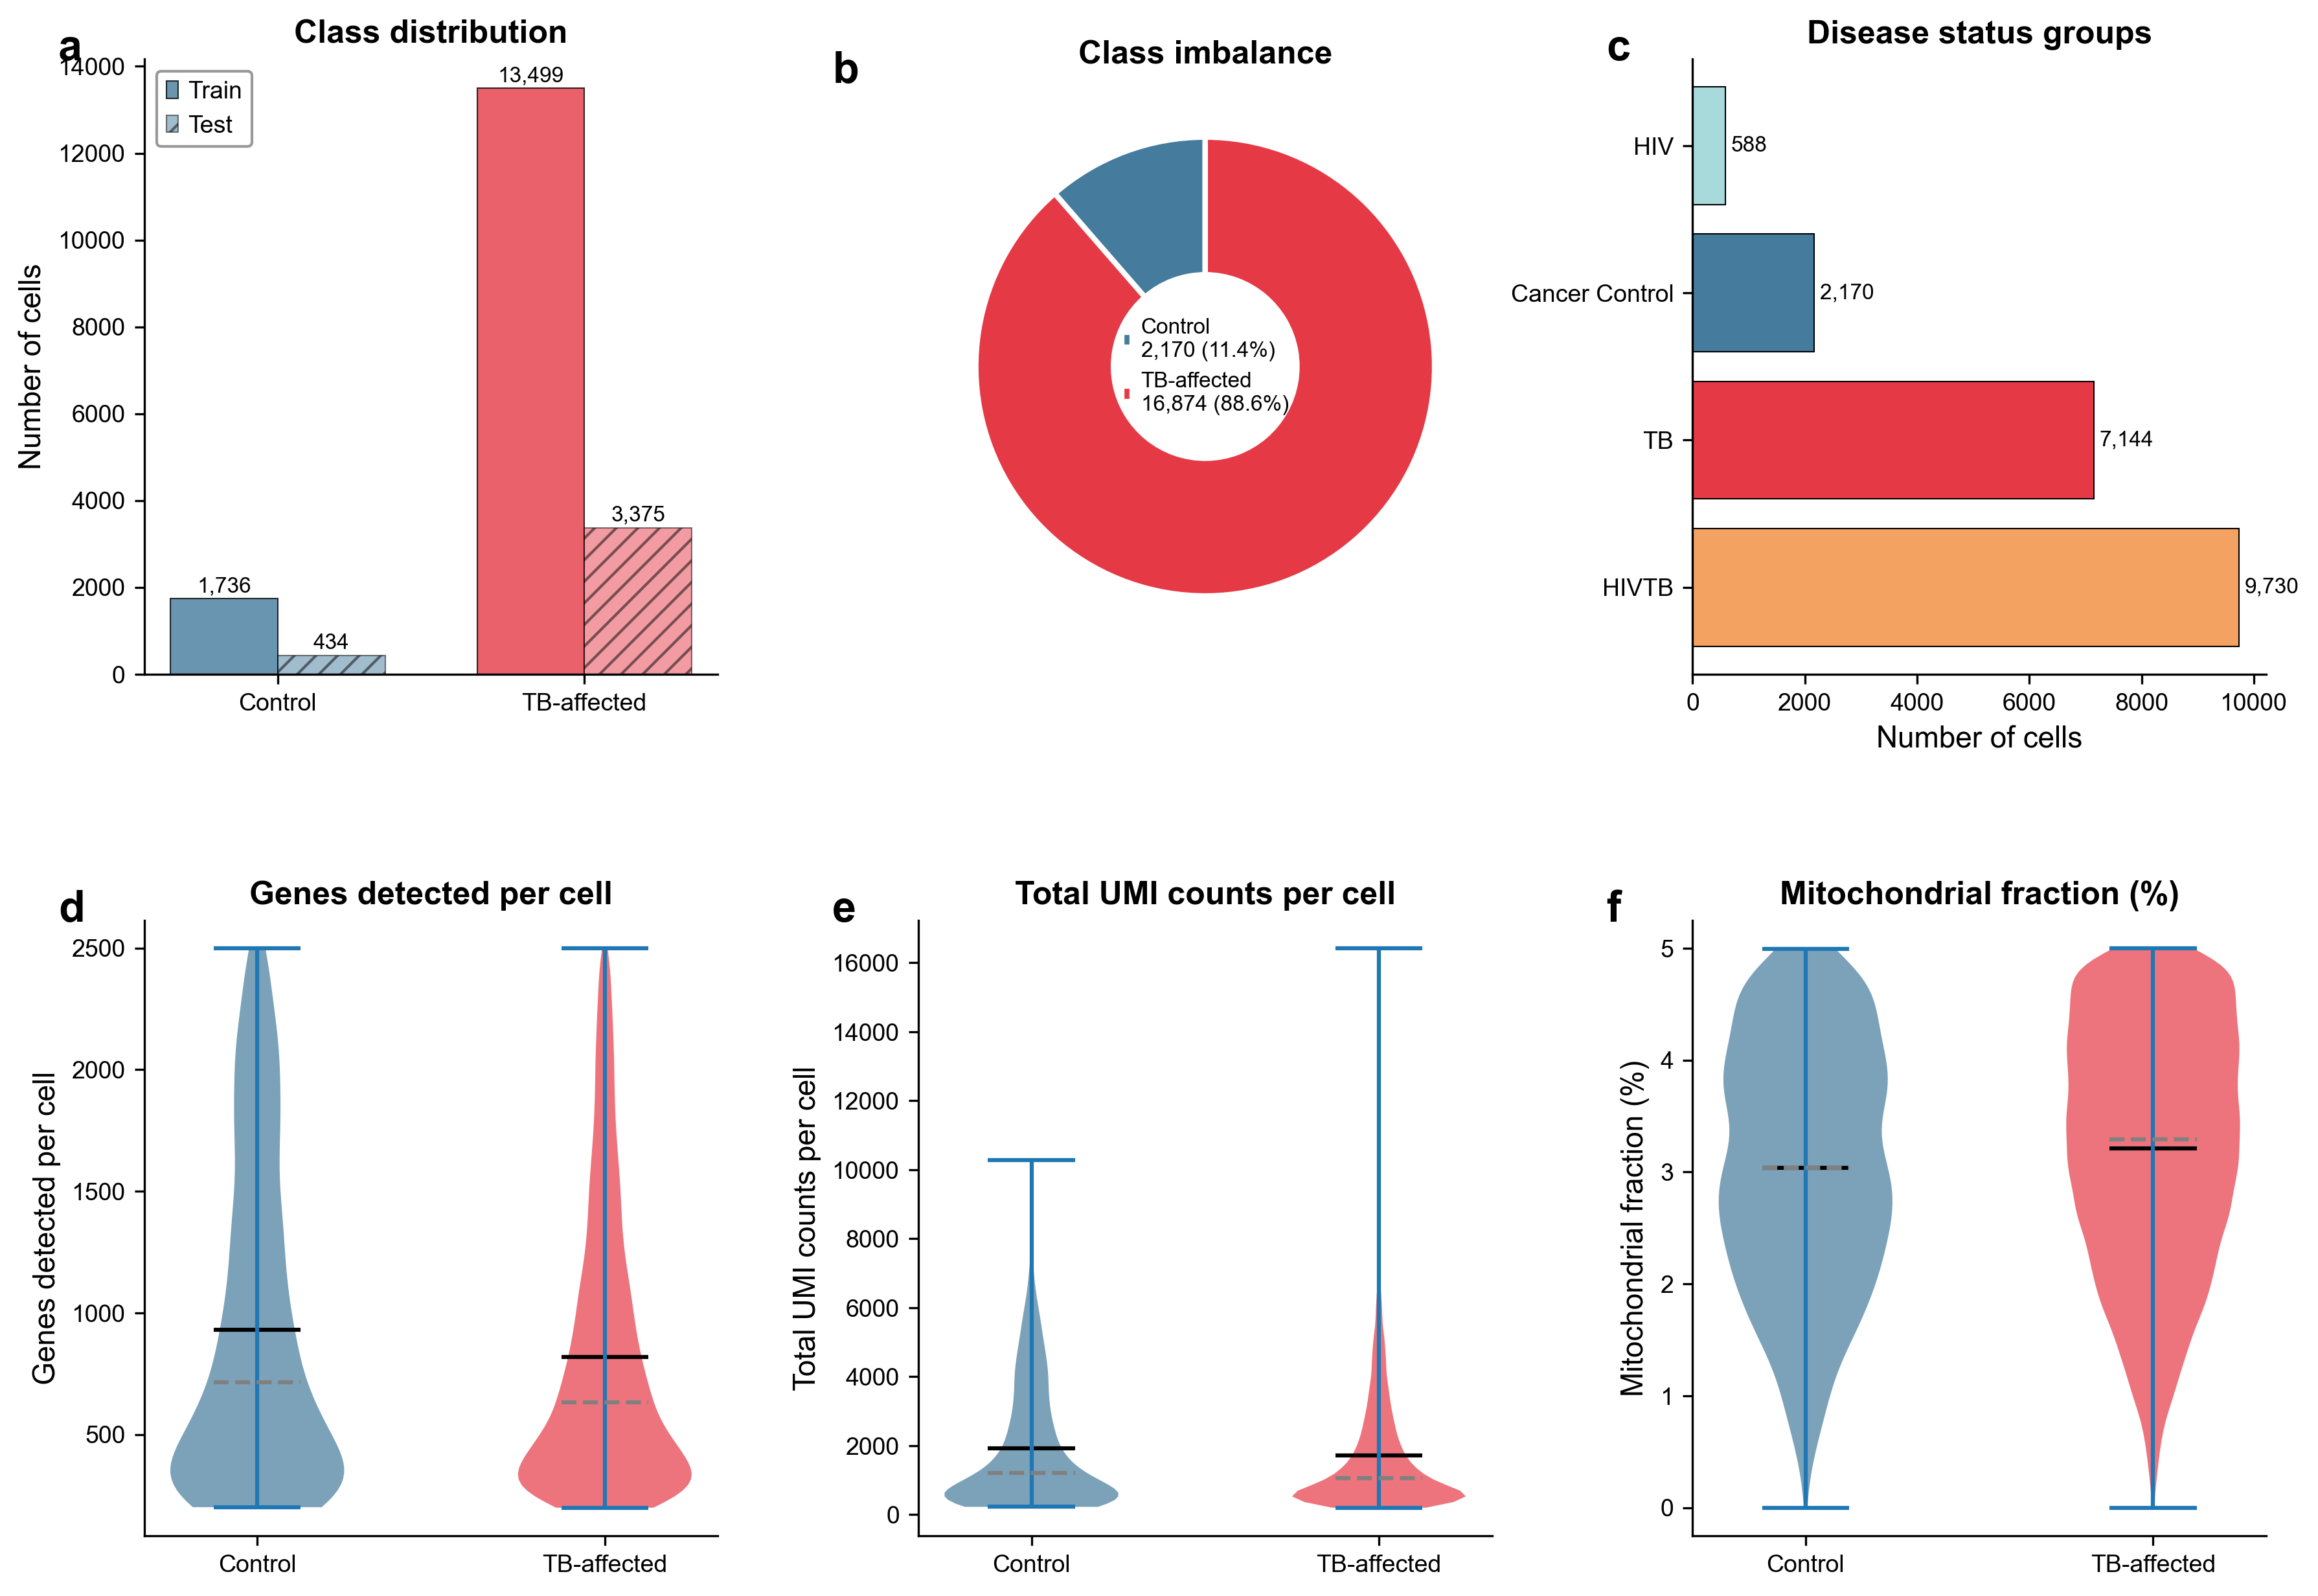
\includegraphics[width=\textwidth]{figure1_data_overview.png}
\caption{\textbf{Dataset overview and quality control.} \textbf{(a)} Class distribution across training and test sets. \textbf{(b)} Overall class proportions: 2,170 Control cells (11.4\%) and 16,874 TB-affected cells (88.6\%). \textbf{(c)} Distribution of cells across the four original disease status categories. HIV-only cells ($n = 588$) were excluded from classification. \textbf{(d--f)} Violin plots comparing quality control metrics between Control and TB-affected cells: genes detected per cell, total UMI counts, and mitochondrial transcript fraction. Solid lines, means; dashed lines, medians.}
\label{fig:overview}
\end{figure}

\subsection*{Dimensionality reduction reveals partial class separation}

Principal component analysis (PCA) on the 2,497 highly variable gene features revealed partial but incomplete separation between Control and TB-affected cells (Fig.~\ref{fig:dimred}a). The first two principal components captured 8.5\% and 5.3\% of the total variance, respectively, and a scree plot showed that 20 PCs accounted for approximately 30\% of the total variance, with a characteristic elbow at PC3 (Fig.~\ref{fig:dimred}b). This distribution of variance across many components indicates that the biological signal is encoded across multiple independent axes of variation rather than concentrated in a single dominant component, a pattern well suited to capture by multivariate machine learning classifiers. The t-distributed stochastic neighbour embedding (t-SNE) applied to the top 20 PCs of a 5,000-cell subsample revealed distinct clusters with partial class separation (Fig.~\ref{fig:dimred}c), confirming that the transcriptomic distinction between granuloma-associated and control cell states requires high-dimensional modelling to fully resolve. A three-dimensional PCA projection of PC1 through PC3 further illustrated that Control cells occupy a compact region of the feature space, while TB-affected cells spread across multiple principal components (Fig.~\ref{fig:dimred}d). This spatial dispersion in three dimensions is consistent with the heterogeneity of immune cell populations within the granuloma microenvironment and underscores the need for ensemble classifiers capable of learning complex, non-linear decision boundaries.

\begin{figure}[!ht]
\centering
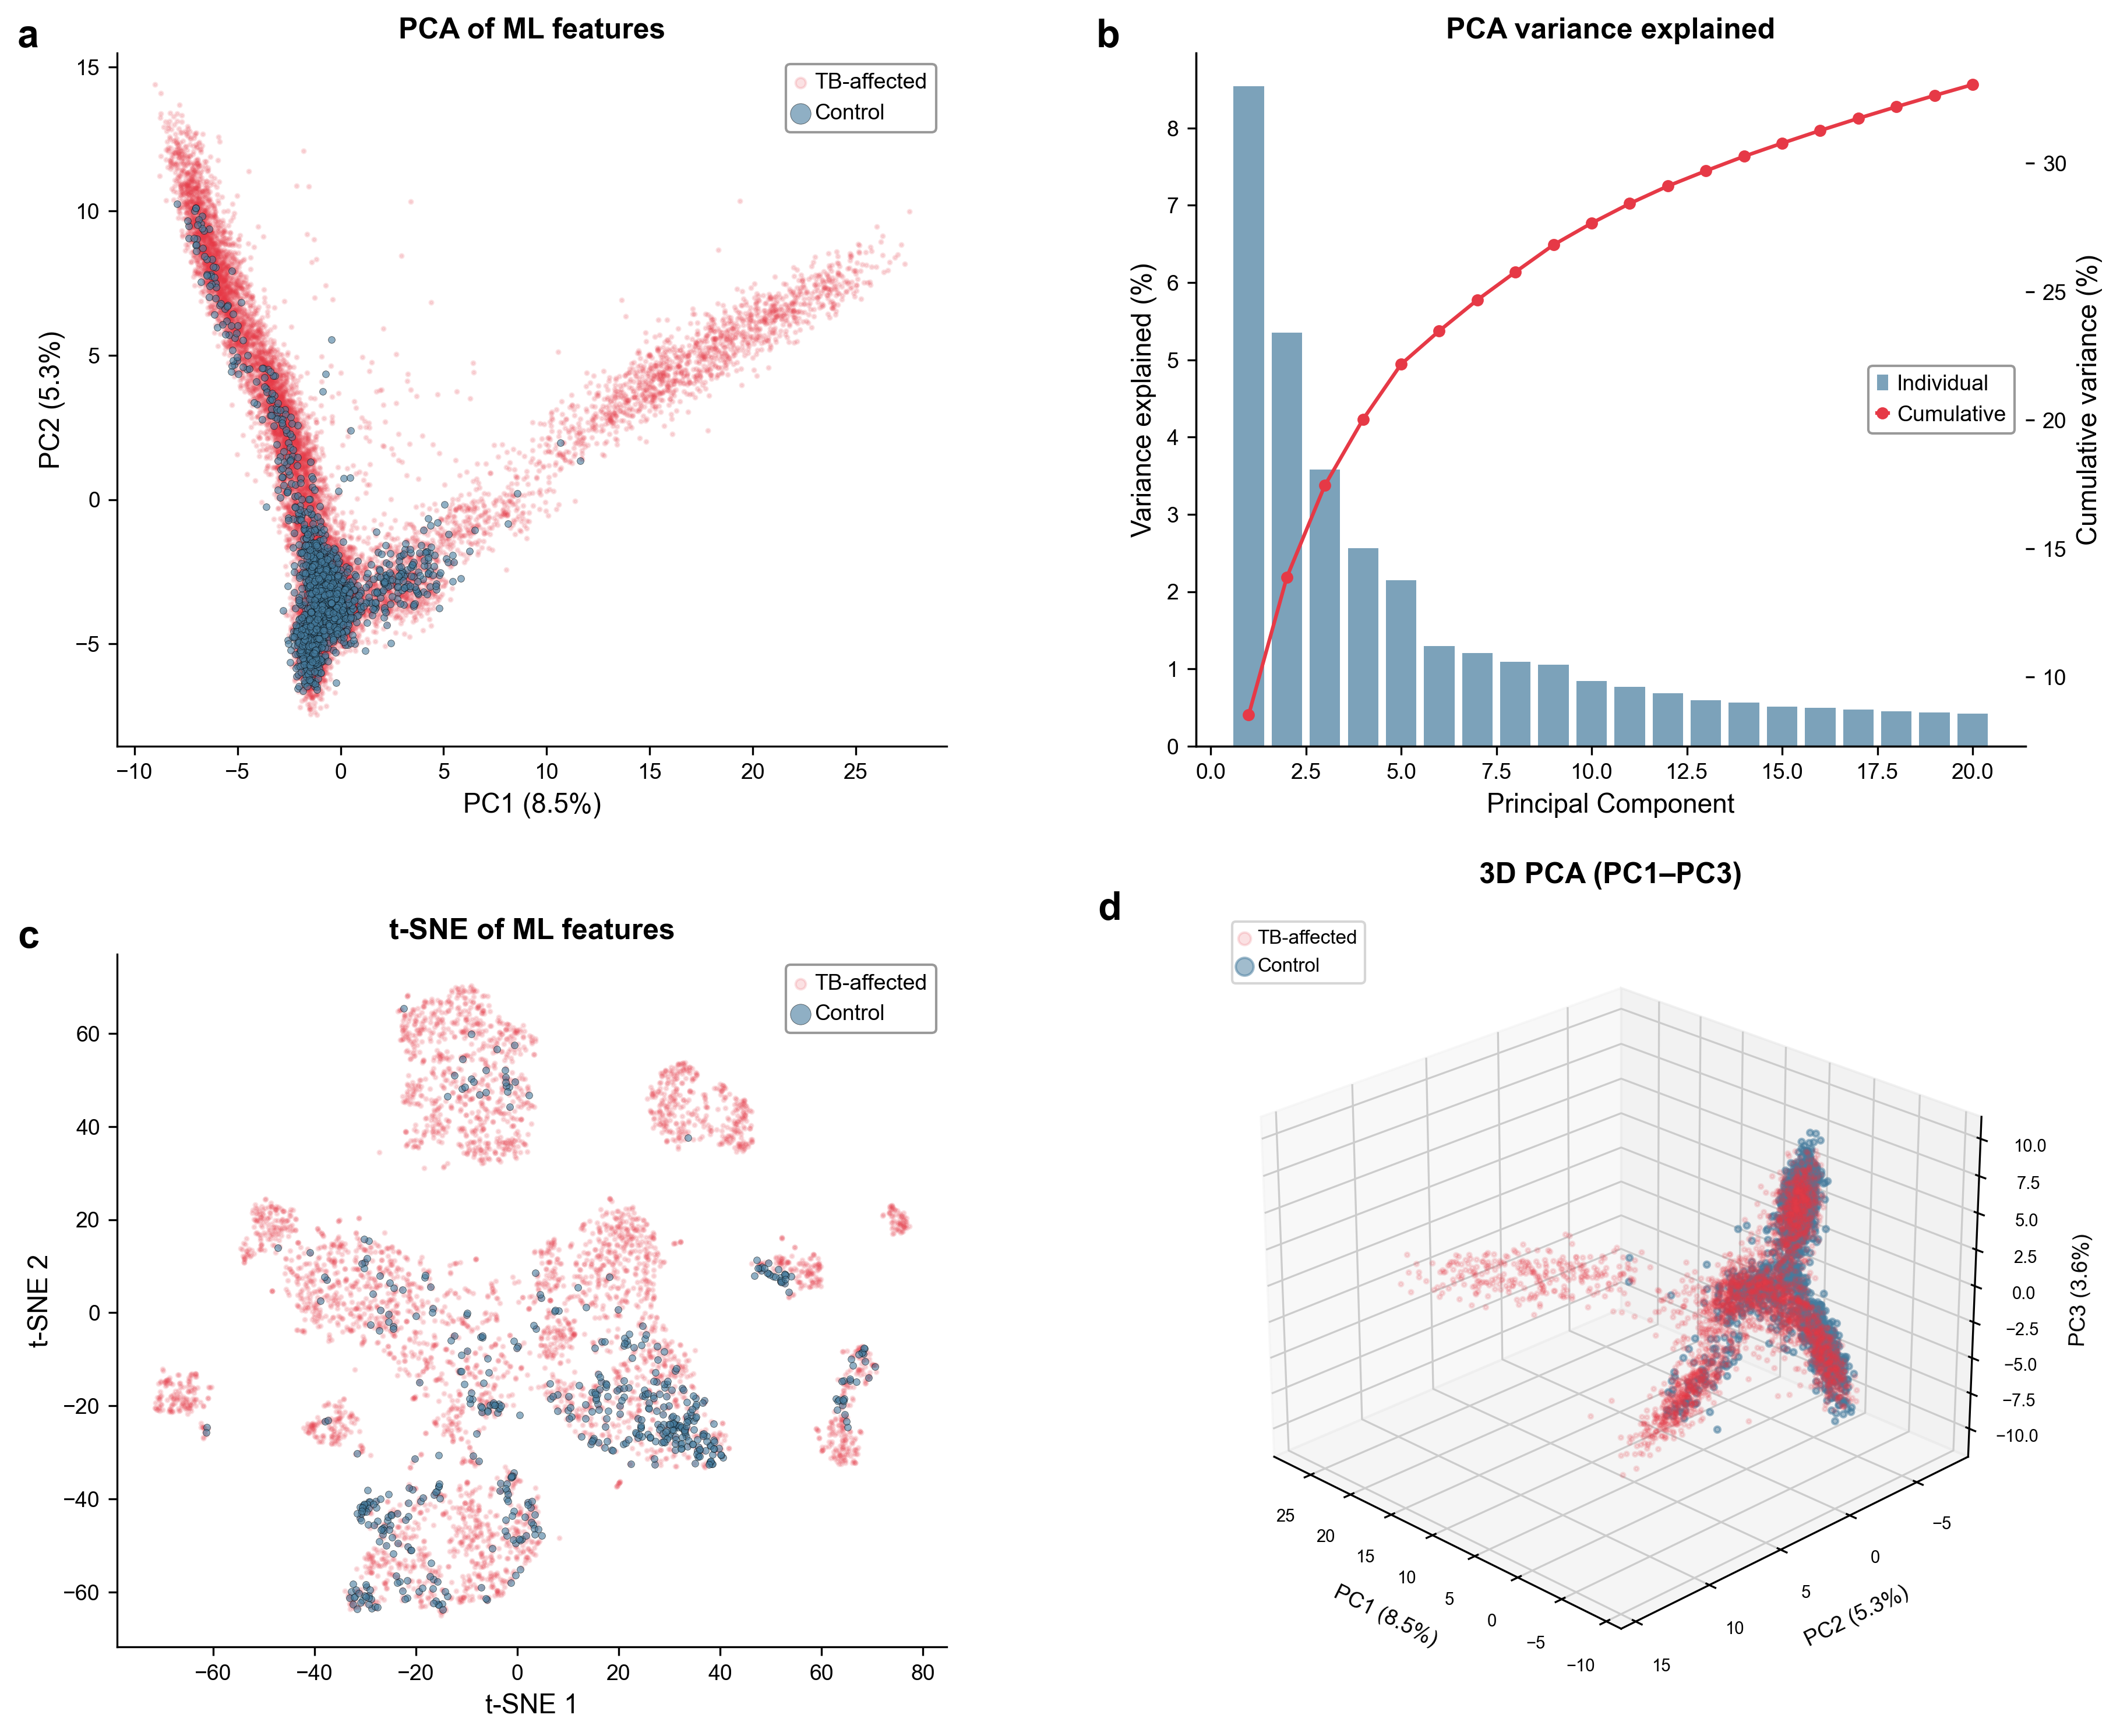
\includegraphics[width=\textwidth]{figure2_dimensionality_reduction.png}
\caption{\textbf{Dimensionality reduction of single-cell transcriptomes.} \textbf{(a)} PCA of the 2,497 highly variable gene features coloured by condition (blue, Control; red, TB-affected). Control cells are plotted on top for visibility. \textbf{(b)} Variance explained by the first 20 principal components (bars, individual; red line, cumulative). \textbf{(c)} t-SNE embedding of a 5,000-cell subsample projected onto the top 20 PCs. \textbf{(d)} Three-dimensional PCA projection (PC1--PC3) showing the spatial distribution of 3,000 subsampled Control and TB-affected cells. Control cells form a compact cluster, while TB-affected cells are dispersed across multiple principal components, reflecting the cellular heterogeneity of the granuloma microenvironment.}
\label{fig:dimred}
\end{figure}

\subsection*{Ensemble classifiers achieve high-accuracy discrimination}

Four classifiers were trained on the full set of 2,497 highly variable gene features: Random Forest, XGBoost, LightGBM, and a stacking ensemble combining the three base learners through logistic regression meta-learning. LightGBM achieved the highest overall discrimination on the held-out test set, with an AUC-ROC of 0.970, an F1 score of 0.969, and balanced precision (0.971) and recall (0.966) (Table~\ref{tab:performance}; Fig.~\ref{fig:performance}a). The stacking ensemble performed comparably (AUC-ROC = 0.968) but did not surpass the best individual model, consistent with the expectation that meta-learning benefits are marginal when a single base learner already approaches ceiling performance\cite{wolpert1992}. Five-fold cross-validation AUC-ROC estimates closely matched test set performance for all models (LightGBM: $0.966 \pm 0.005$; Fig.~\ref{fig:performance}d), indicating minimal overfitting.

Confusion matrices revealed complementary error profiles (Fig.~\ref{fig:performance}c). Random Forest exhibited the highest recall (0.991) but the lowest precision (0.936), correctly identifying nearly all TB-affected cells while misclassifying 227 of 434 Control cells as TB-affected. The stacking ensemble showed the opposite pattern, achieving the highest precision (0.987) at the expense of reduced recall (0.915). LightGBM achieved the best balance, correctly classifying 338 of 434 Control cells and 3,260 of 3,375 TB-affected cells. These complementary error profiles confirm that the four models capture partially distinct decision boundaries, and that LightGBM provides the most clinically useful trade-off between sensitivity and specificity for this classification task.

\begin{table}[!ht]
\centering
\caption{\textbf{Model performance on the held-out test set ($n = 3{,}809$ cells).} Best values in each column are in bold.}
\label{tab:performance}
\begin{tabular}{lccccc}
\toprule
\textbf{Model} & \textbf{Accuracy} & \textbf{F1} & \textbf{Precision} & \textbf{Recall} & \textbf{AUC-ROC} \\
\midrule
Random Forest      & 0.932 & 0.963 & 0.936 & \textbf{0.991} & 0.944 \\
XGBoost            & 0.917 & 0.952 & 0.978 & 0.927 & 0.962 \\
\textbf{LightGBM}  & \textbf{0.945} & \textbf{0.969} & 0.971 & 0.966 & \textbf{0.970} \\
Stacking Ensemble  & 0.913 & 0.949 & \textbf{0.987} & 0.915 & 0.968 \\
\bottomrule
\end{tabular}
\end{table}

\begin{figure}[!ht]
\centering
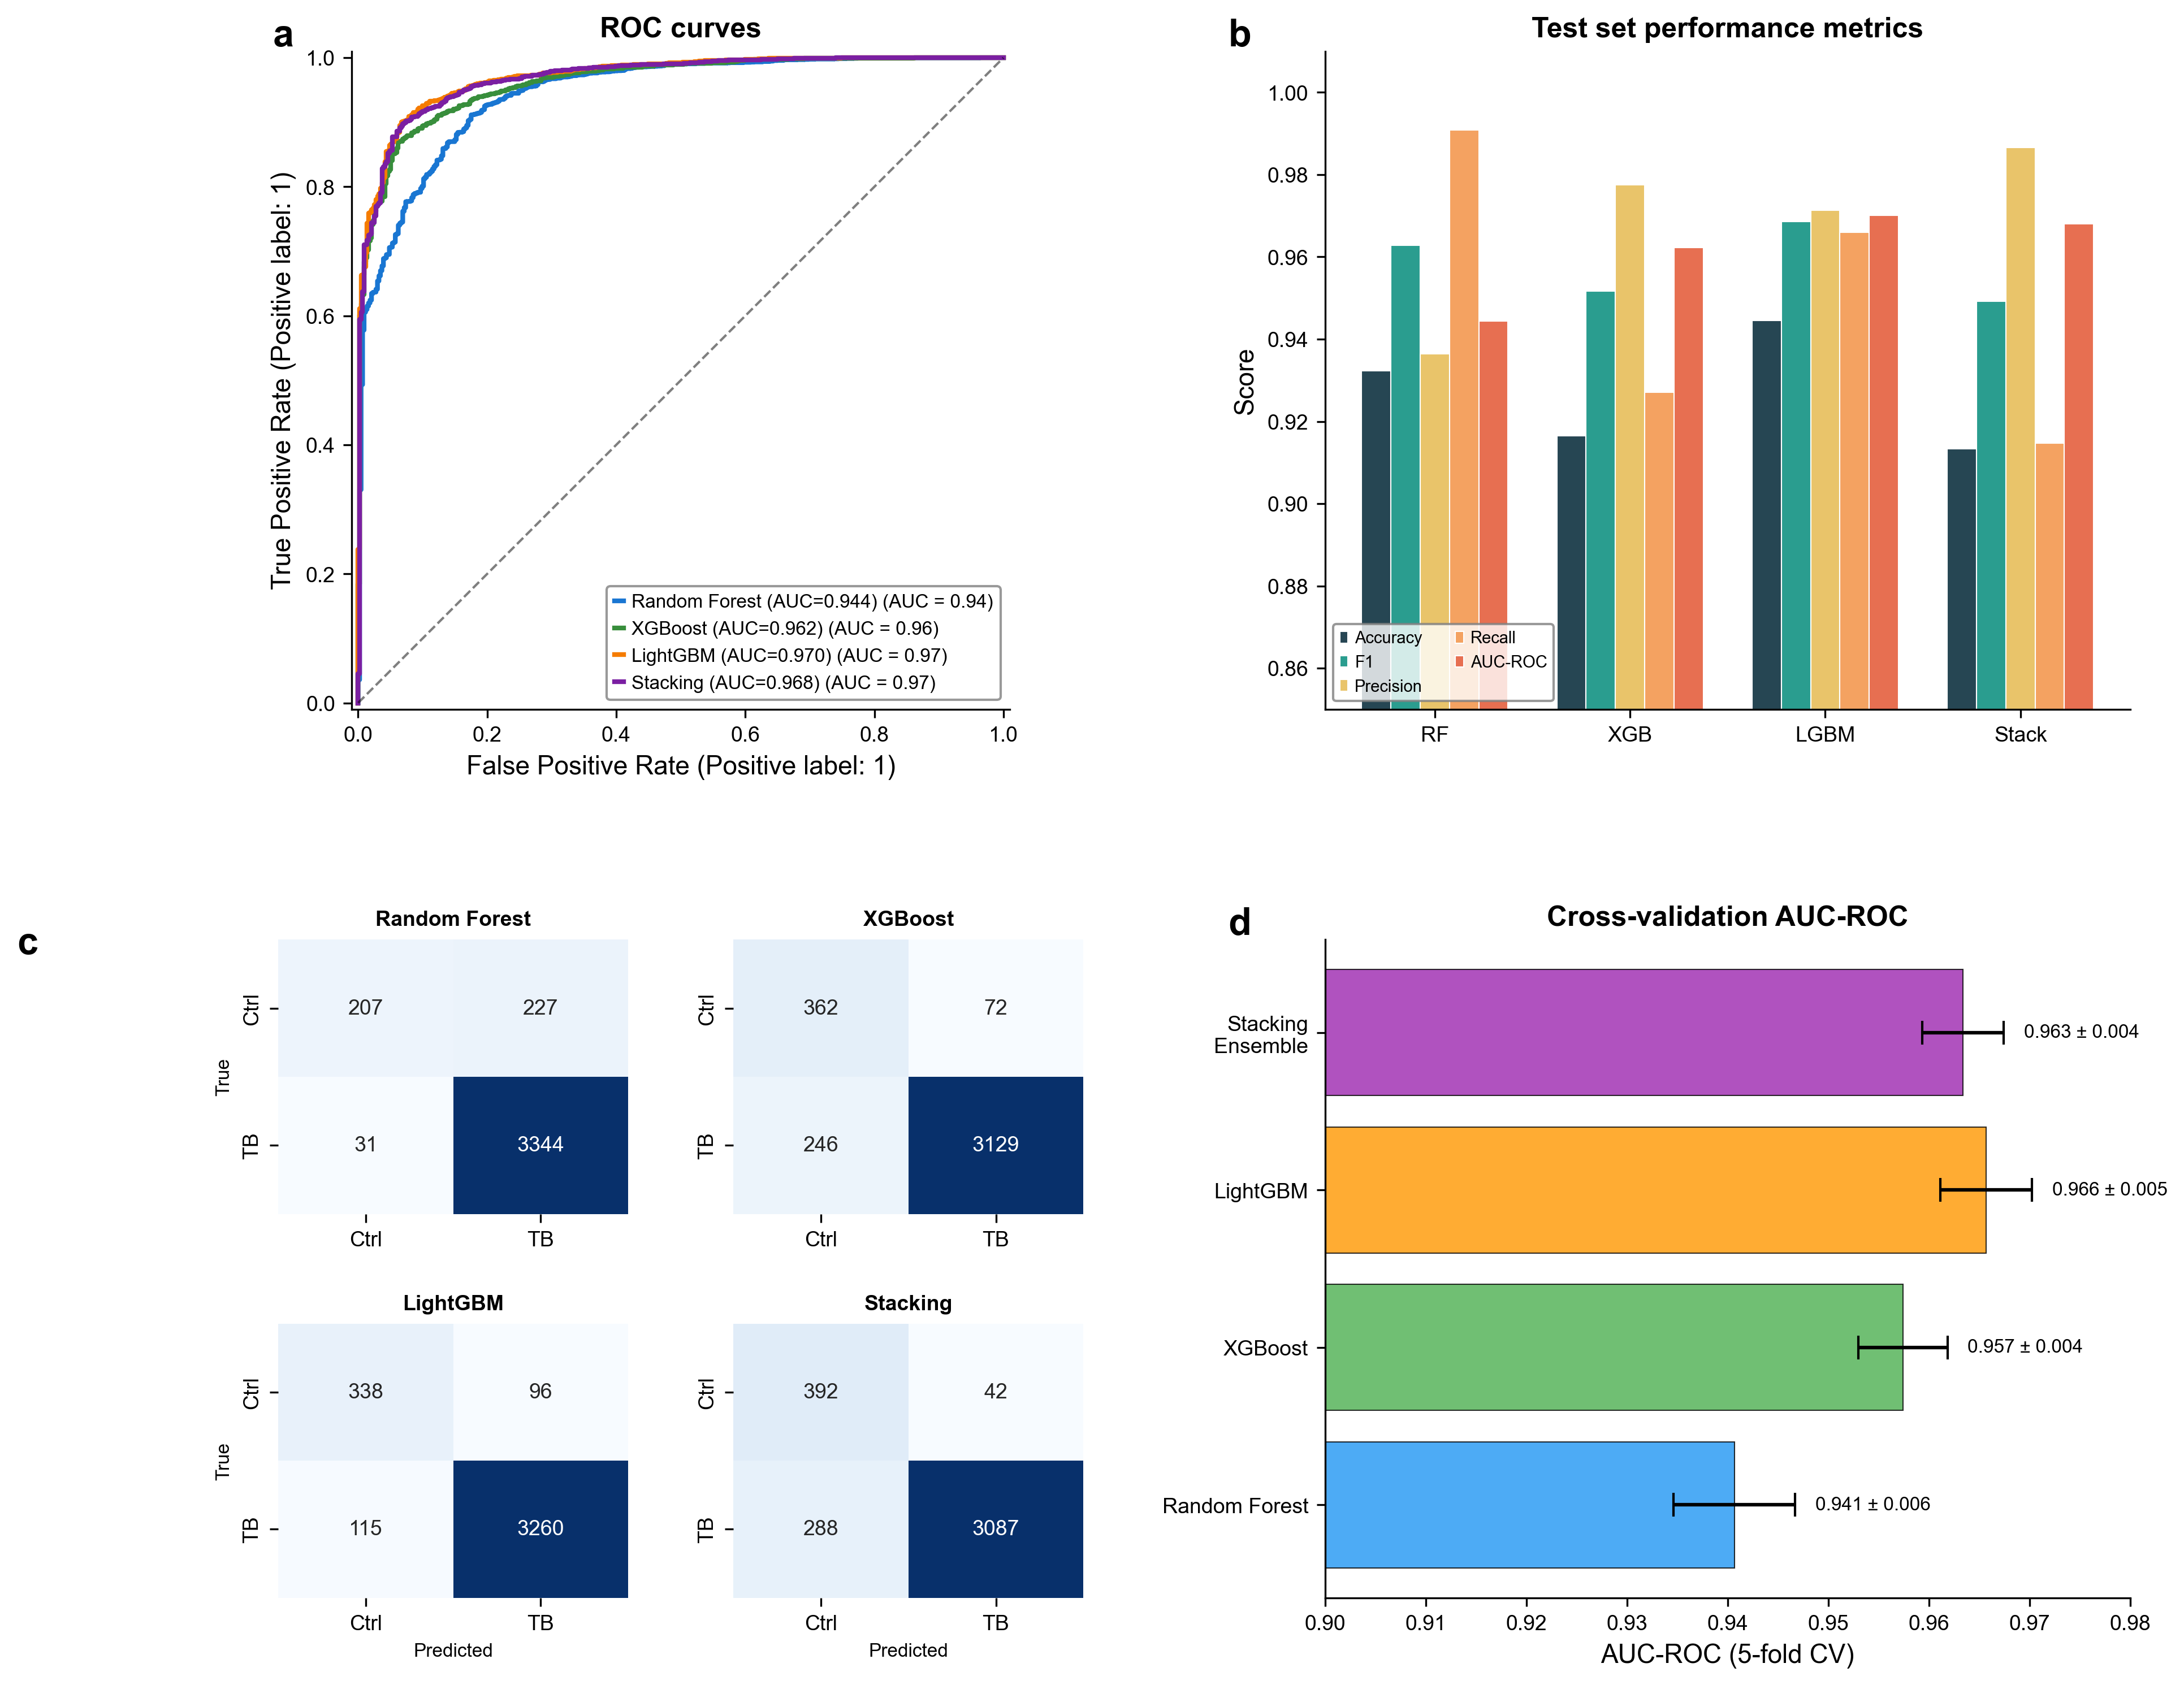
\includegraphics[width=\textwidth]{figure3_model_performance.png}
\caption{\textbf{Ensemble machine learning model performance.} \textbf{(a)} ROC curves for all four classifiers on the held-out test set. The dashed diagonal indicates random performance (AUC = 0.500). \textbf{(b)} Multi-metric comparison across models. \textbf{(c)} Confusion matrices for each classifier, showing complementary error profiles. \textbf{(d)} Five-fold cross-validation AUC-ROC with error bars (one standard deviation).}
\label{fig:performance}
\end{figure}

\subsection*{Hyperparameter tuning does not improve baseline performance}

To evaluate whether systematic hyperparameter optimization could further improve classification performance, Bayesian optimization was applied using Optuna with a Tree-structured Parzen Estimator sampler across all four models. For each classifier, key hyperparameters were tuned over 50 trials using five-fold cross-validated AUC-ROC as the objective. The search spaces included the number of estimators (100--500), maximum depth (3--15), learning rate (0.01--0.3), and regularization parameters specific to each algorithm. Table~\ref{tab:tuning} compares the held-out test set AUC-ROC for the baseline (default) and tuned configurations.

\begin{table}[!ht]
\centering
\caption{\textbf{Comparison of baseline and tuned model AUC-ROC on the held-out test set.} All four models showed marginal performance decreases after hyperparameter optimization.}
\label{tab:tuning}
\begin{tabular}{lccc}
\toprule
\textbf{Model} & \textbf{Baseline AUC} & \textbf{Tuned AUC} & \textbf{$\Delta$AUC} \\
\midrule
Random Forest     & 0.944 & 0.926 & $-$0.019 \\
XGBoost           & 0.962 & 0.961 & $-$0.001 \\
LightGBM          & 0.970 & 0.967 & $-$0.003 \\
Stacking Ensemble & 0.968 & 0.964 & $-$0.004 \\
\bottomrule
\end{tabular}
\end{table}

All four models exhibited marginal performance decreases following tuning, with Random Forest showing the largest decline ($\Delta$AUC = $-$0.019) and XGBoost remaining essentially unchanged ($\Delta$AUC = $-$0.001). This outcome indicates that the default hyperparameter configurations of these well-established libraries are already well suited to the structure of single-cell transcriptomic data, which is characterized by moderate dimensionality (2,497 features), substantial sample size ($n = 15{,}235$ training cells), and relatively clear class boundaries. The observation that tuning did not improve performance also argues against overfitting in the baseline models, as aggressive optimization would be expected to yield gains primarily through memorization of noise in the training data. Based on these results, the baseline configurations were retained for all subsequent analyses.

\subsection*{SHAP analysis identifies a 100-gene TB disease signature}

To identify the specific genes driving classification, SHAP values were computed for LightGBM using TreeExplainer\cite{lundberg2020} on a subsample of 2,000 test cells. The top 100 genes ranked by mean absolute SHAP value were designated as the TB disease signature; 59 of these were upregulated and 41 were downregulated in TB-affected cells relative to controls (Fig.~\ref{fig:signature}a,b).

The highest-ranked gene, \textit{MTRNR2L12}, is a nuclear-encoded pseudogene derived from mitochondrial 16S rRNA that was downregulated in TB-affected cells (mean $|$SHAP$|$ = 0.449). Its prominence reflects the pronounced mitochondrial transcriptional dysregulation reported in TB-infected macrophages, where mitochondrial stress activates innate immune signalling through the cGAS-STING pathway\cite{wiens2018}. Among the top upregulated genes, \textit{TAOK1} (thousand-and-one amino acid kinase 1), ranked second, is a MAP3K family member that phosphorylates p38 MAPK and JNK, placing it at a critical node in the stress-activated kinase cascade that governs inflammatory cytokine production in myeloid cells\cite{raman2007}. (The third-ranked gene, \textit{RGS2}, is discussed below with the downregulated signature genes.) \textit{S100A12} (calgranulin C), ranked fourth, encodes a calcium-binding protein with direct antimicrobial activity against intracellular mycobacteria that is induced by IFN-$\gamma$ and TLR2/1 ligands in human macrophages\cite{realegeno2016}. \textit{COL3A1}, ranked fifth, and \textit{DCN}, ranked tenth, are extracellular matrix components whose presence corroborates recent spatial transcriptomic evidence that TB granulomas undergo active fibrotic remodelling\cite{scp3227}. \textit{CTSL} (cathepsin L), ranked sixth, encodes a lysosomal cysteine protease central to phagosome maturation and MHC class II antigen processing\cite{gideon2022,honey2003}. \textit{CCL18}, ranked seventh, is produced by alternatively activated macrophages and recruits naive T cells to sites of chronic pulmonary inflammation\cite{koth2004,schutyser2002}. \textit{HLA-DRB5}, ranked eighth, encodes an MHC class II molecule involved in antigen presentation to CD4$^{+}$ T cells, consistent with the active adaptive immune engagement within the granuloma. \textit{FBLN1} (fibulin 1), ranked ninth, is a secreted glycoprotein that modulates extracellular matrix assembly and complements the fibrotic remodelling signal captured by \textit{COL3A1} and \textit{DCN}.

A volcano-style visualization confirmed clear separation between genes with high importance and positive mean SHAP values (upregulated in TB) versus those with negative values (downregulated; Fig.~\ref{fig:signature}c). Functional annotation of the top 30 signature genes showed that immune and inflammatory mediators, metabolism and stress response genes, and extracellular matrix components together accounted for the majority of the predictive signal (Fig.~\ref{fig:signature}d).

\begin{figure}[!ht]
\centering
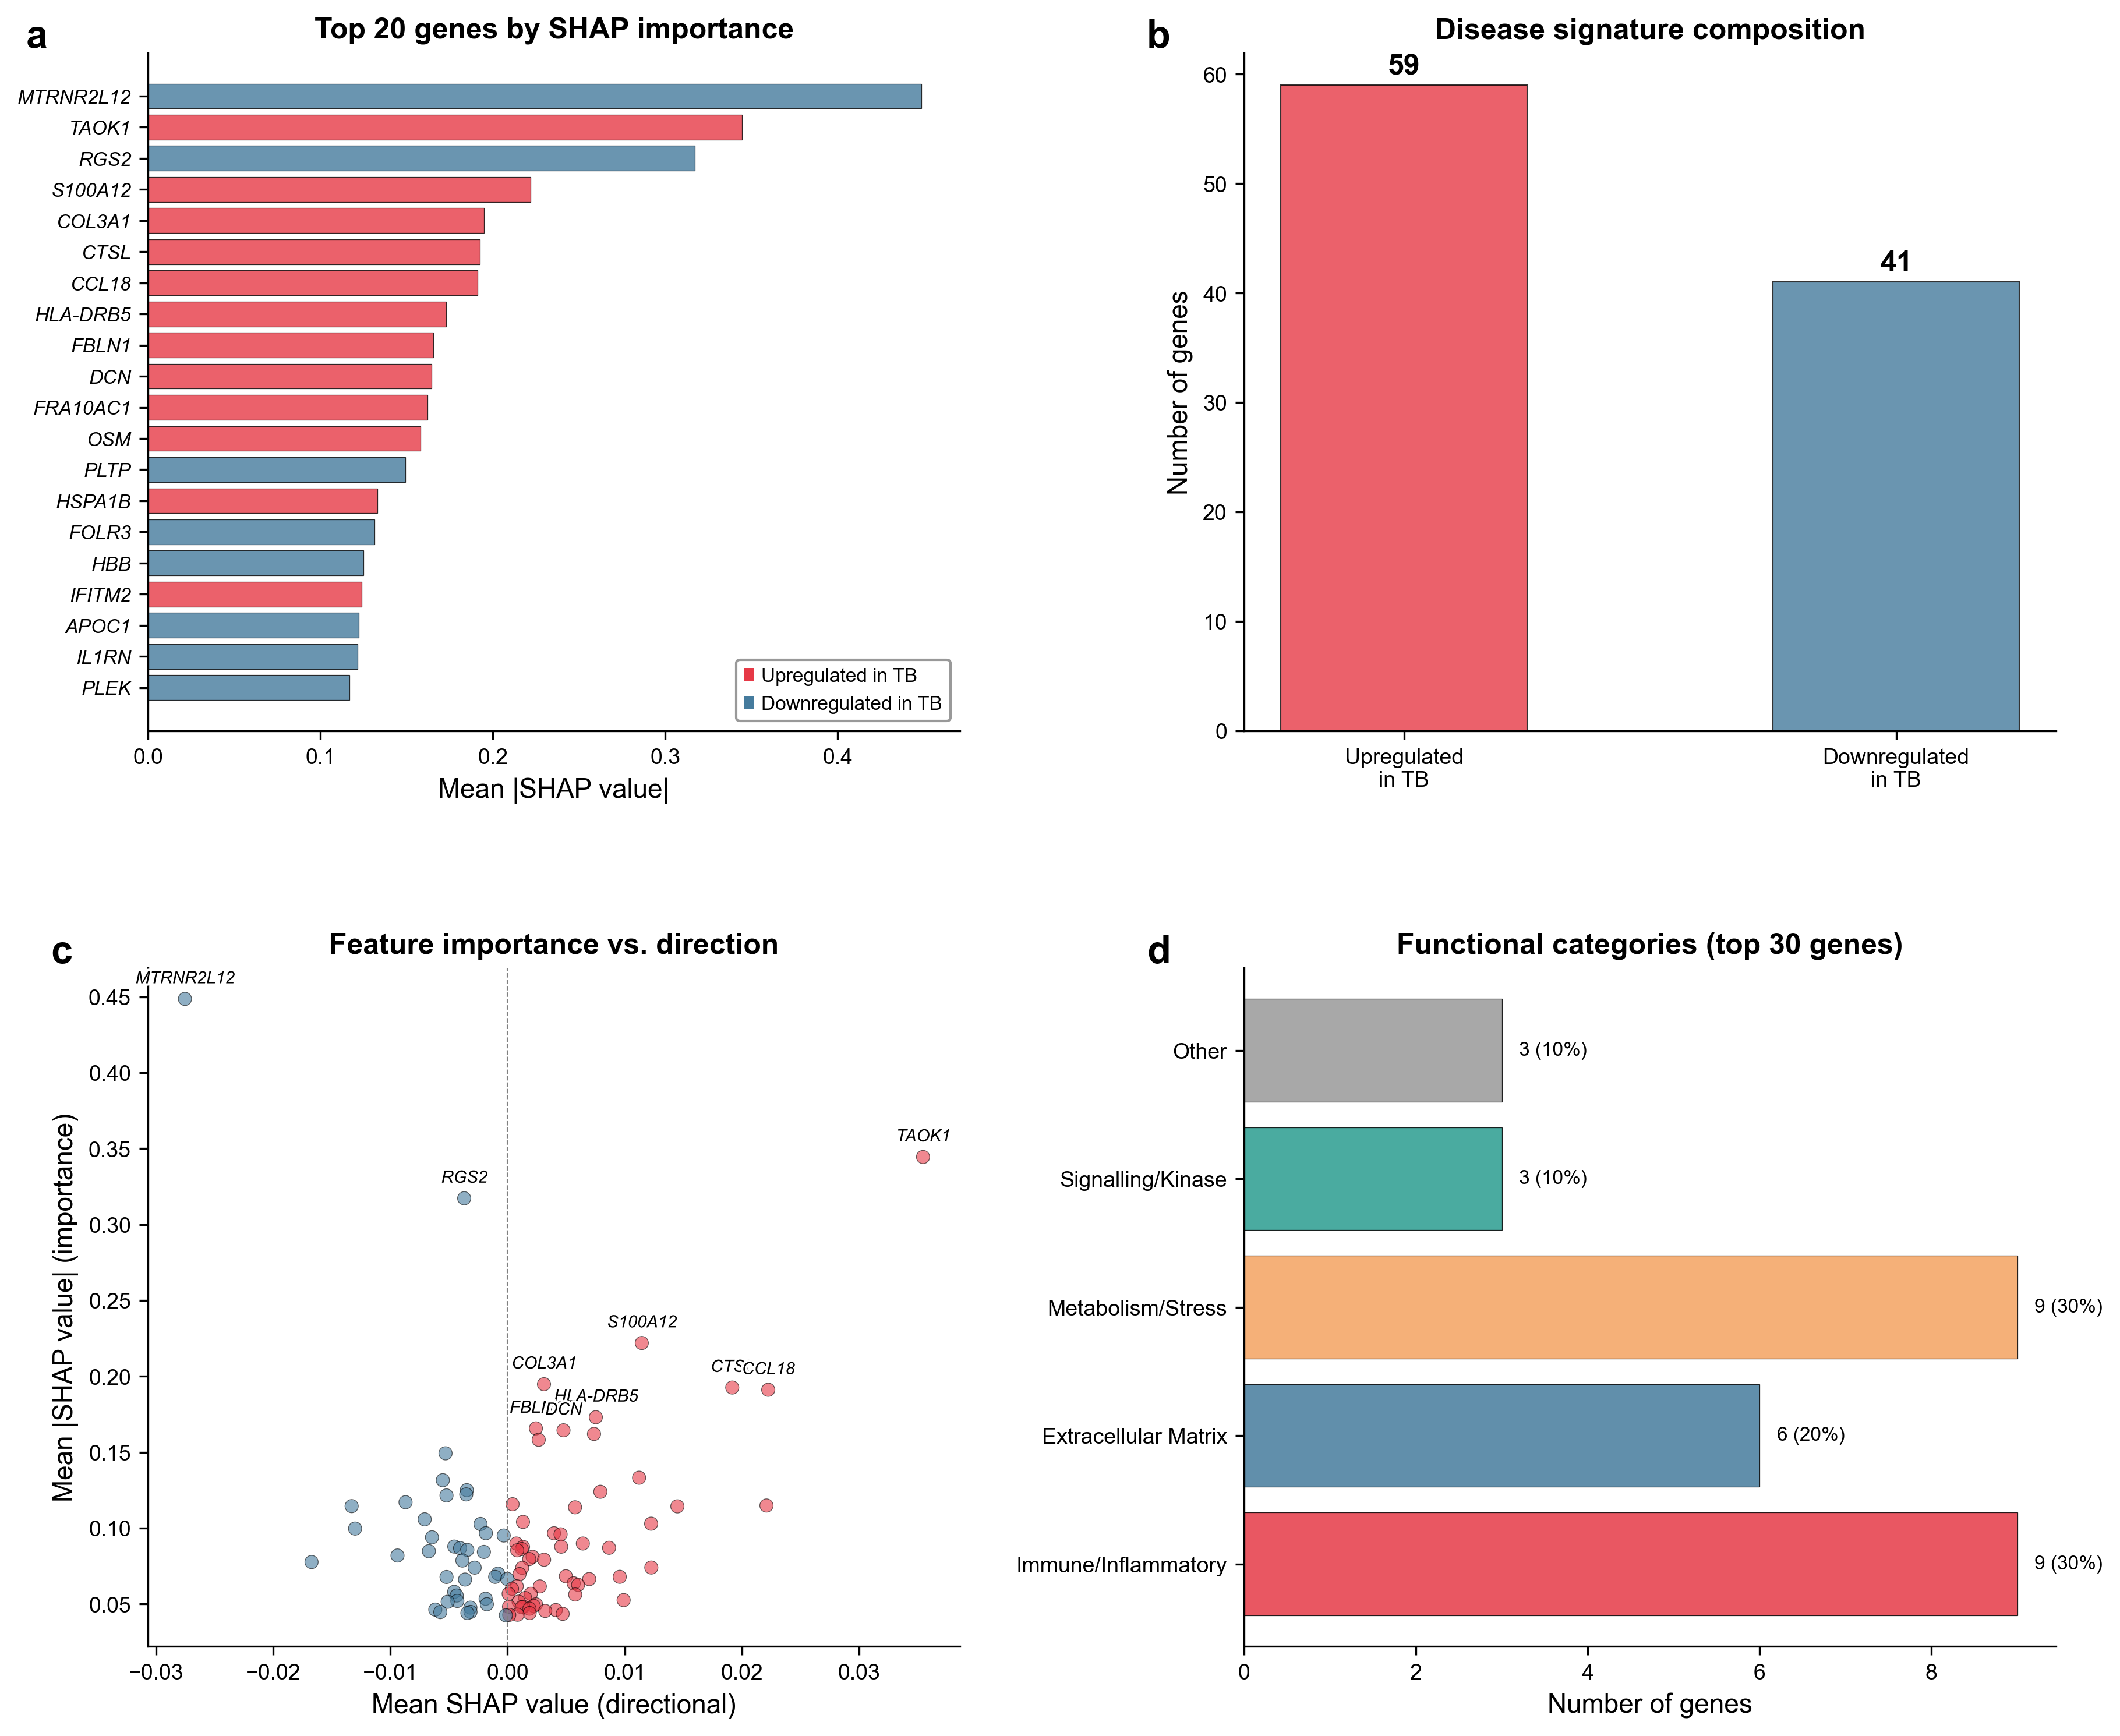
\includegraphics[width=\textwidth]{figure4_disease_signature.png}
\caption{\textbf{SHAP-derived TB disease signature.} \textbf{(a)} Top 20 genes ranked by mean absolute SHAP value. Red, upregulated in TB; blue, downregulated. \textbf{(b)} Composition of the 100-gene signature. \textbf{(c)} Volcano-style plot of mean SHAP value (directional) versus mean absolute SHAP value (importance) for all 100 signature genes. \textbf{(d)} Functional categorization of the top 30 signature genes.}
\label{fig:signature}
\end{figure}

Among the downregulated signature genes, \textit{RGS2} (regulator of G-protein signalling 2), the third most important feature overall, attenuates chemokine receptor signalling in leukocytes; its suppression in the granuloma may reflect sustained chemotactic activation of infiltrating immune cells\cite{bowman2015}. \textit{PLTP} (phospholipid transfer protein) and \textit{APOC1} (apolipoprotein C-I), both downregulated, participate in lipid metabolism and lipoprotein remodelling, consistent with the metabolic reprogramming of granuloma macrophages toward a lipid-laden, foamy phenotype that favours mycobacterial persistence\cite{peyron2008}. Pairwise correlations among the top 15 signature genes revealed an extracellular matrix module (\textit{COL3A1}, \textit{DCN}, \textit{FBLN1}; pairwise $r > 0.65$) and a lipid transport module (\textit{CTSL}, \textit{PLTP}, \textit{CCL18}; pairwise $r = 0.41$--$0.48$), while most signature genes showed weak mutual correlations (Supplementary Fig.~S1), confirming that the model captures largely independent biological programmes.

\subsection*{Expression patterns confirm directionality of the disease signature}

A z-scored expression heatmap for the top 30 SHAP genes across a balanced subsample of 200 Control and 200 TB-affected cells revealed a block-diagonal structure (Fig.~\ref{fig:heatmap}). The top-ranked gene, \textit{MTRNR2L12}, showed higher expression in control cells, confirming its downregulation in TB-affected cells. Upregulated genes such as \textit{TAOK1}, \textit{S100A12}, and \textit{CCL18} showed elevated expression predominantly in TB-affected cells, while downregulated genes such as \textit{RGS2}, \textit{PLTP}, and \textit{FOLR3} exhibited higher expression in controls. The expression patterns were not uniform across all TB-affected cells, reflecting the known cellular diversity within the granuloma microenvironment\cite{scp3227}.

\begin{figure}[!ht]
\centering
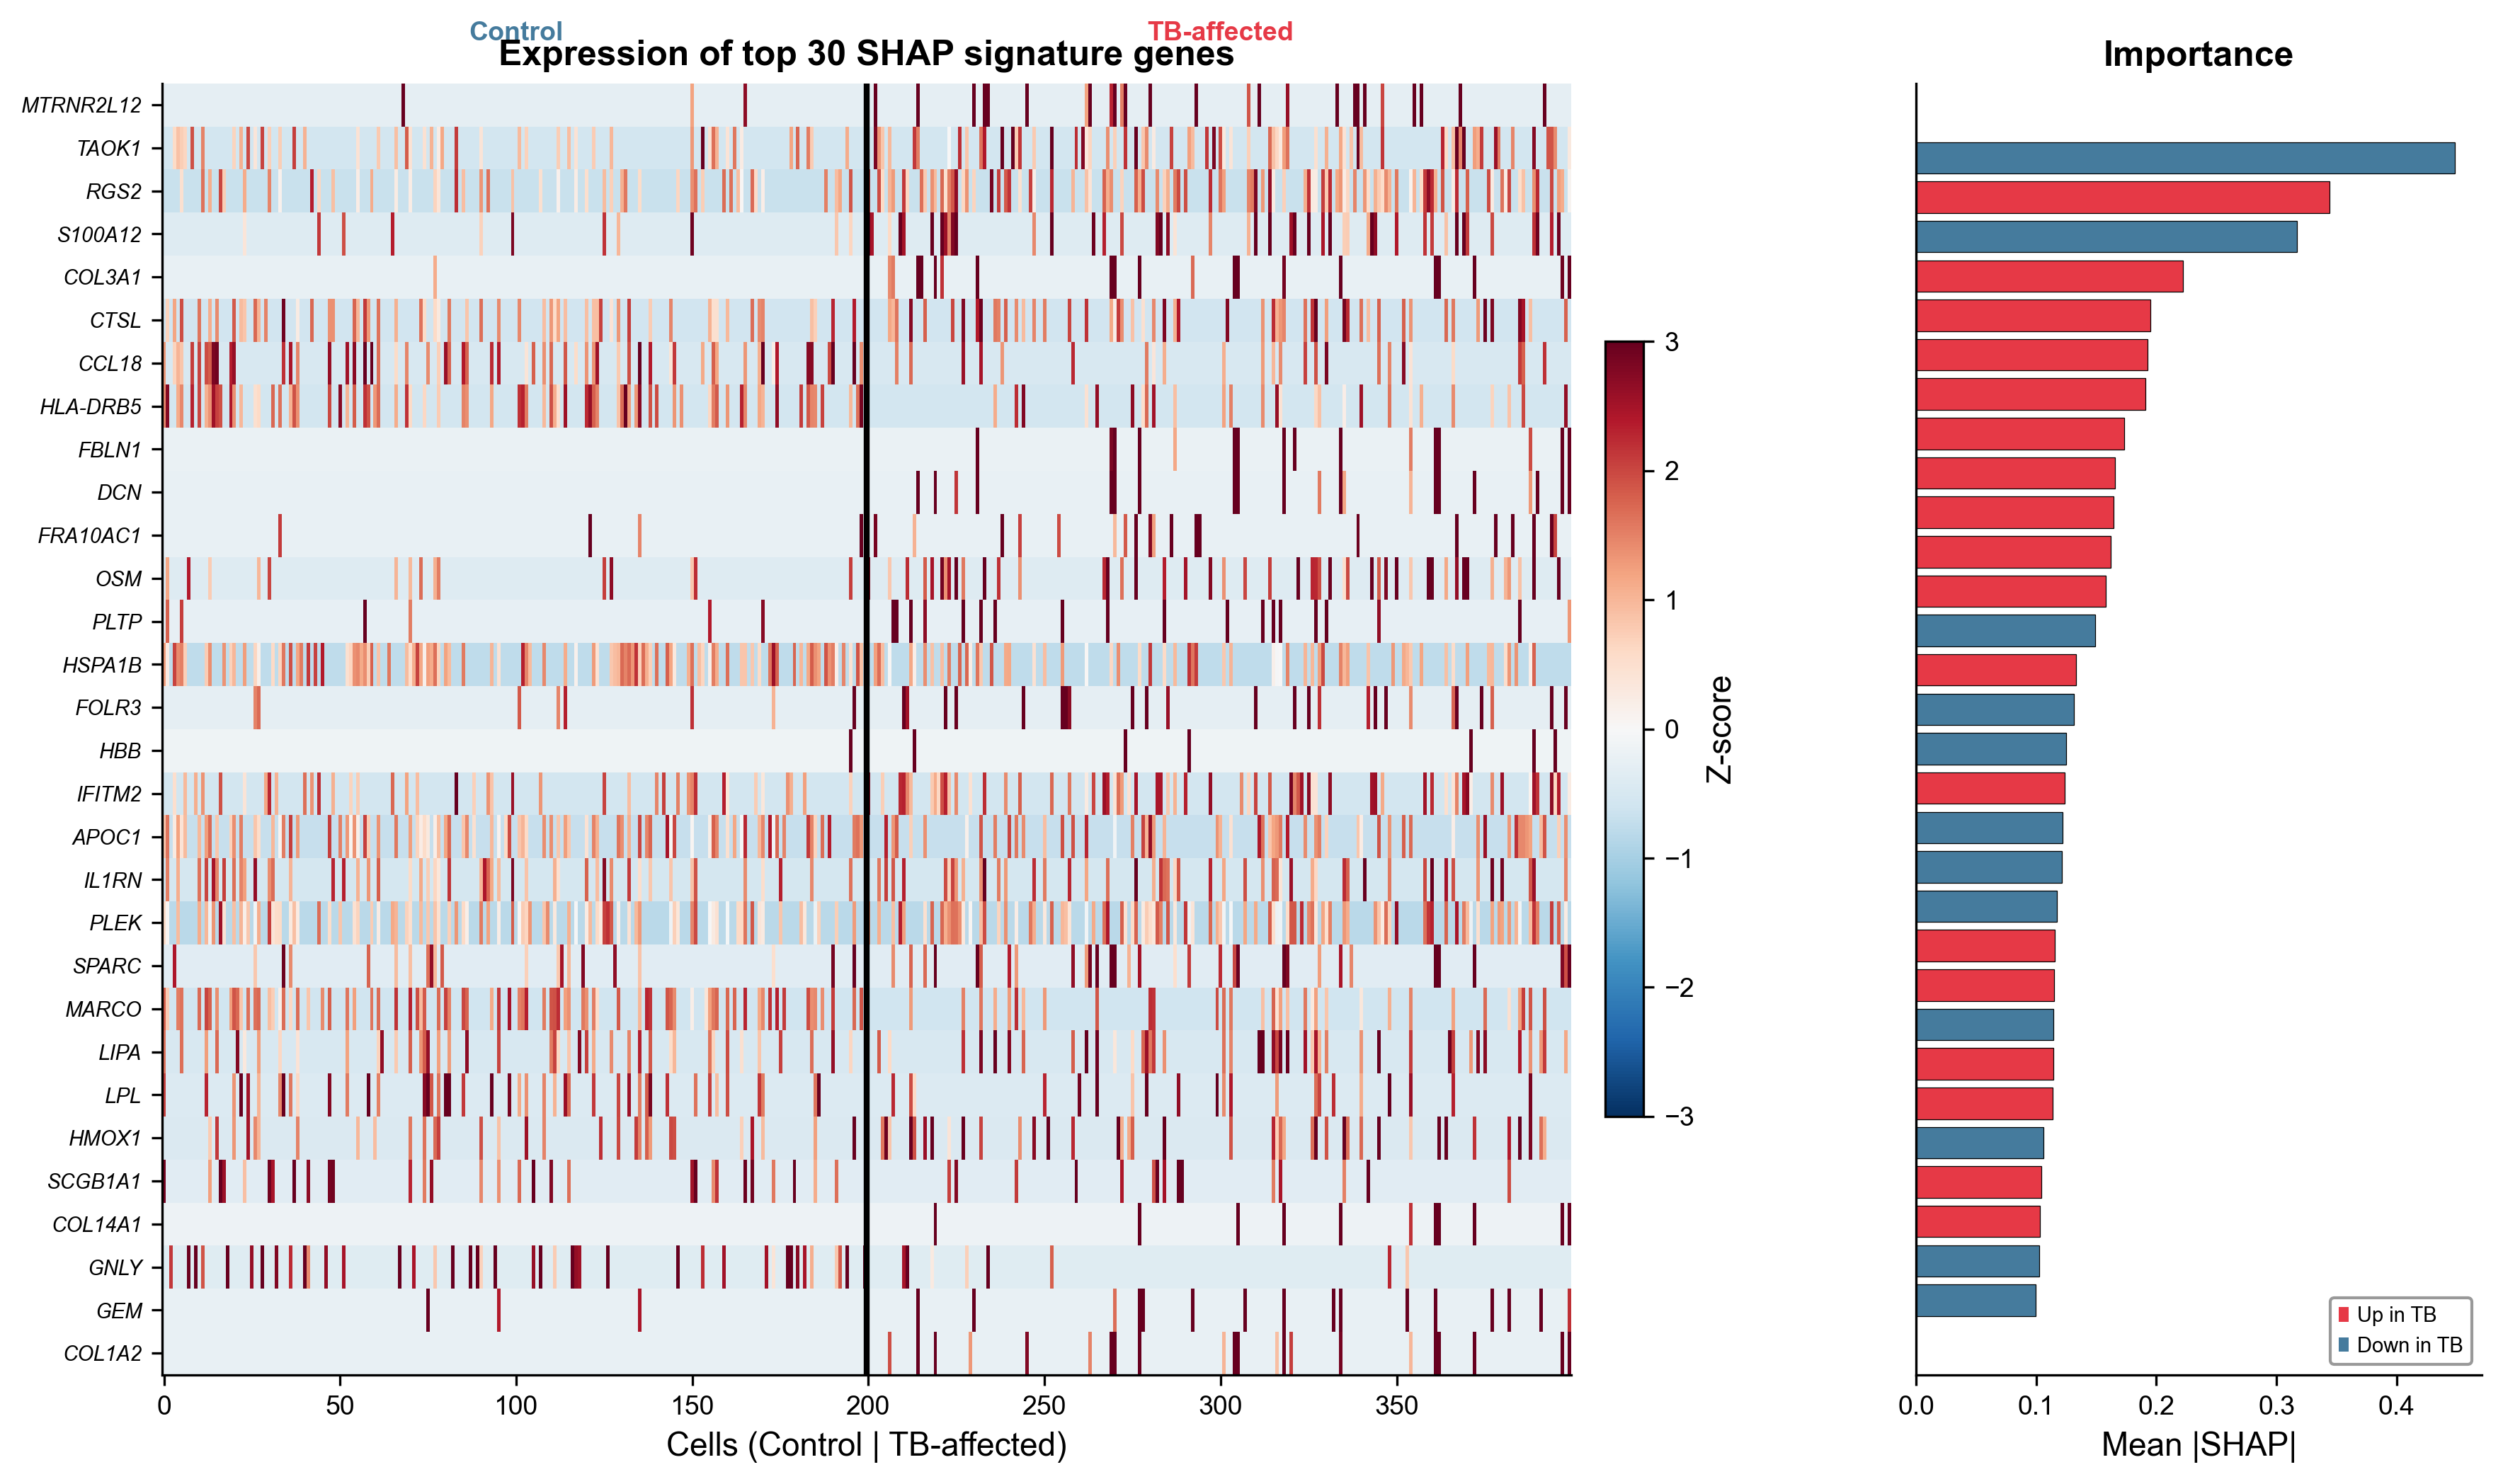
\includegraphics[width=\textwidth]{figure5_expression_heatmap.png}
\caption{\textbf{Expression heatmap of the top 30 SHAP signature genes.} Z-scored expression (clipped to $\pm$3) for 200 Control (left) and 200 TB-affected (right) cells, separated by the vertical black line. Gene names are ordered by SHAP importance. The right panel shows the mean absolute SHAP value for each gene (red, upregulated in TB; blue, downregulated).}
\label{fig:heatmap}
\end{figure}

\subsection*{Connectivity mapping nominates host-directed drug candidates}

The L1000 Connectivity Map\cite{subramanian2017} was queried with the 59 upregulated and 41 downregulated signature genes, seeking compounds whose perturbation profiles inversely correlated with the disease signature. This analysis returned 1,831 compounds at adjusted $P < 0.05$, of which 979 passed $P < 0.01$ and 208 achieved $P < 0.0001$ (Fig.~\ref{fig:drugs}c). The top-ranked candidate by combined enrichment score was adenosine triphosphate (Fig.~\ref{fig:drugs}a), consistent with the established role of purinergic signalling in macrophage activation and mycobacterial killing. Monensin, a polyether ionophore antibiotic with demonstrated antimycobacterial activity, ranked second. Tracazolate, a GABA$_{\text{A}}$ receptor modulator with anti-inflammatory properties, ranked third. Cephaeline and anisomycin, both protein synthesis inhibitors, and prochlorperazine, a phenothiazine with demonstrated activity against intracellular bacteria, appeared among the top six candidates. The enrichment score distribution showed that most significant hits clustered at lower scores, while a small number achieved both high scores and extreme statistical significance (Fig.~\ref{fig:drugs}b,d). The convergence of compounds with known anti-inflammatory, immunomodulatory, or direct antimicrobial mechanisms among the top candidates provides independent validation that the disease signature captures biologically relevant pathways amenable to pharmacological intervention.

\begin{figure}[!ht]
\centering
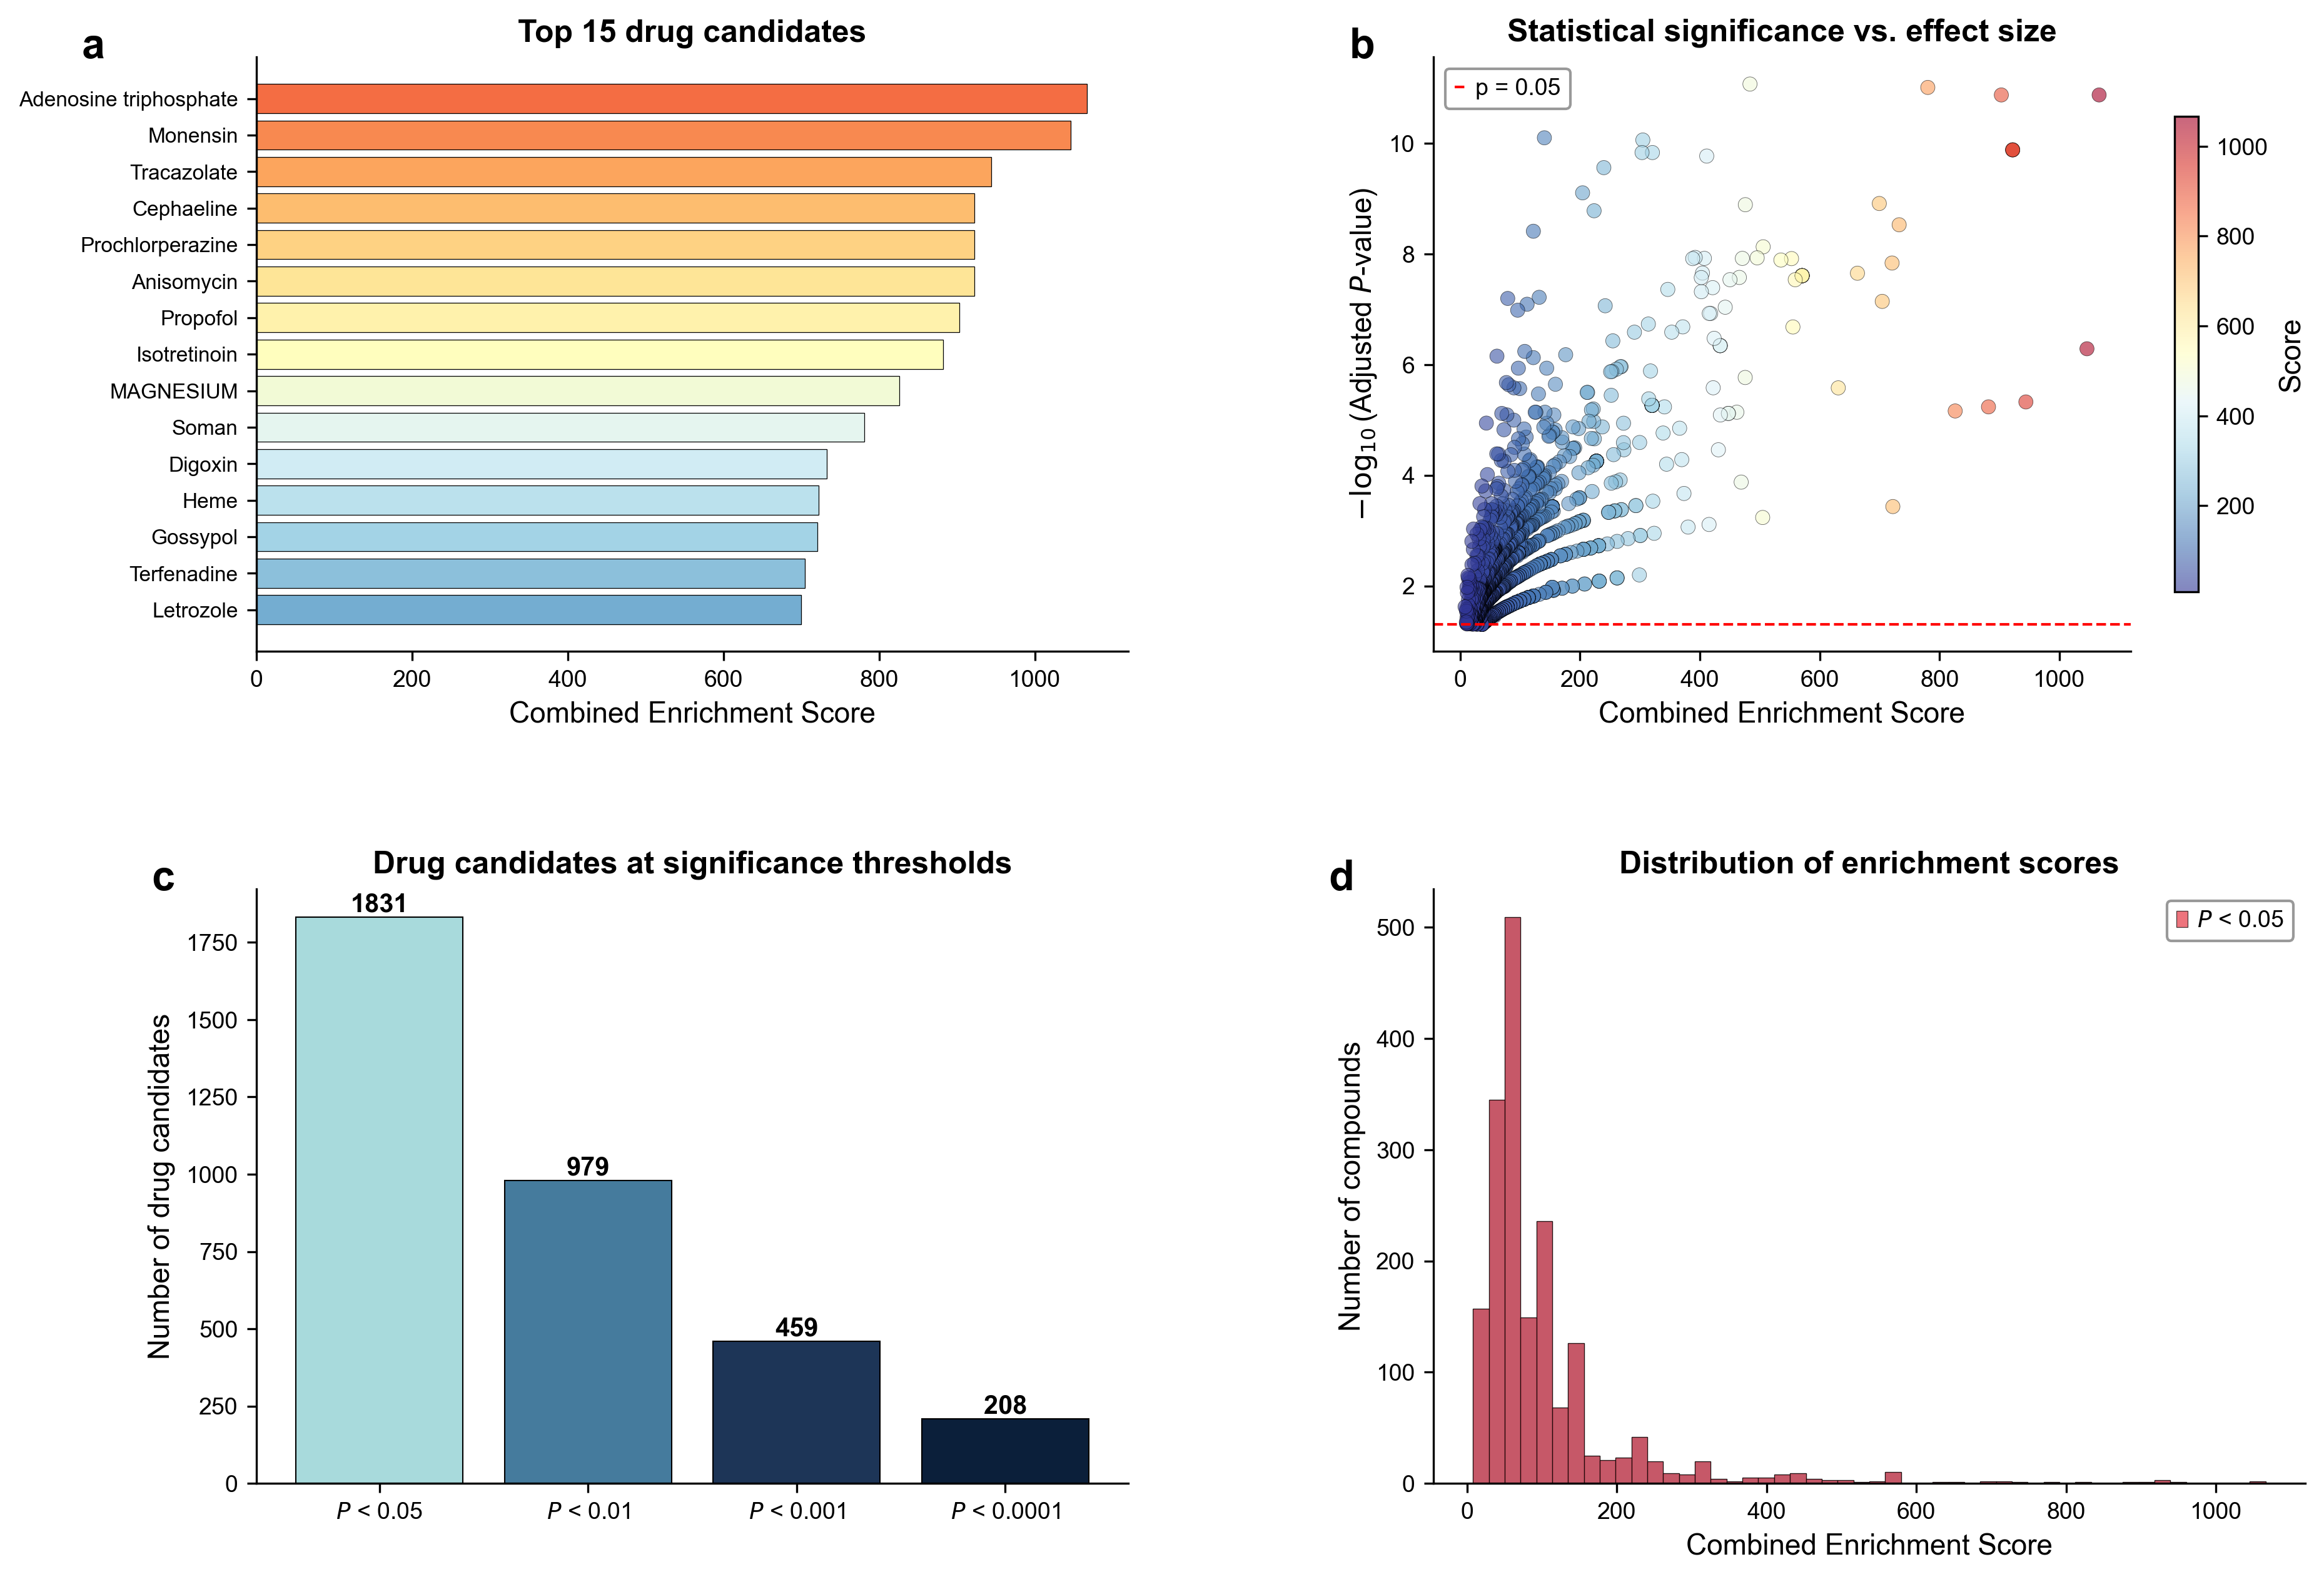
\includegraphics[width=\textwidth]{figure6_drug_repurposing.png}
\caption{\textbf{Computational drug repurposing analysis.} \textbf{(a)} Top 15 drug candidates ranked by combined enrichment score. \textbf{(b)} Combined enrichment score versus $-\log_{10}$(adjusted $P$-value) for all compounds. Dashed red line, $P = 0.05$. \textbf{(c)} Number of significant candidates at progressively stringent thresholds. \textbf{(d)} Distribution of enrichment scores; significant hits ($P < 0.05$) in red.}
\label{fig:drugs}
\end{figure}

% ============================================================
% DISCUSSION (1000--1500 words)
% ============================================================
\section*{Discussion}

In this study, it is demonstrated that ensemble machine learning applied to single-cell transcriptomes from human TB lung granulomas of South African patients simultaneously achieves high-accuracy cell-state classification and yields a biologically interpretable disease signature with direct therapeutic implications. The LightGBM classifier discriminated TB-affected from control cells with an AUC-ROC of 0.970, and the SHAP-derived 100-gene signature recapitulated known TB immunopathology while identifying potentially actionable therapeutic targets.

The biological coherence of the disease signature strengthens confidence in its validity. The prominence of \textit{S100A12} and \textit{CCL18} among the top-ranked genes aligns with the established roles of calgranulin-mediated antimicrobial defence and alternative macrophage activation in TB granulomas\cite{realegeno2016,koth2004}. The identification of extracellular matrix genes (\textit{COL3A1}, \textit{DCN}, \textit{FBLN1}) among the most predictive features is consistent with the emerging recognition that granuloma fibrosis, mediated by myofibroblast populations, contributes to the structural remodelling that both contains and shelters \textit{M.~tuberculosis}\cite{scp3227}. The observation that most signature genes exhibit weak pairwise correlations indicates that the ensemble classifier captures multiple biologically independent programmes rather than a single co-regulated module, which would limit the interpretive value of the signature.

The drug repurposing analysis provides a proof-of-concept for translating disease signatures into therapeutic hypotheses. The identification of monensin, a polyether ionophore with documented antimycobacterial properties, and digoxin, a cardiac glycoside whose derivatives have demonstrated anti-mycobacterial activity in macrophage infection models, among the top 15 candidates provides pharmacological plausibility for the approach. Beyond the top 15, the broader pool of 1,831 significant candidates includes several compounds with independent preclinical evidence supporting host-directed activity against TB. Imatinib\cite{napier2016}, a tyrosine kinase inhibitor, enhances macrophage bactericidal capacity by promoting phagolysosome acidification. Metformin\cite{singhal2014,degner2018} potentiates autophagy-mediated mycobacterial clearance. Verapamil, a calcium channel blocker, has been shown to inhibit bacterial efflux pumps and potentiate bedaquiline activity against drug-resistant TB\cite{gupta2013,adams2011}. Corticosteroids, represented in the candidate list through dexamethasone-related perturbation profiles, have demonstrated clinical benefit in tuberculous meningitis\cite{thwaites2004}. The convergence of computationally nominated candidates with drugs possessing independent experimental support for anti-TB activity provides strong validation of the connectivity mapping approach.

Several limitations of this study merit consideration. First, the classification task distinguishes cells from TB-positive versus TB-negative donors rather than infected versus bystander cells within a single individual; future studies incorporating spatial resolution or infection reporters would enable finer-grained dissection of the within-granuloma transcriptional landscape. Second, the substantial class imbalance (88.6\% TB-affected cells) was addressed through algorithmic class-weight adjustment and stratified sampling, but future work would benefit from experimental designs achieving more balanced representation of disease and control states. Third, the drug repurposing analysis relies on transcriptomic connectivity mapping, which identifies compounds that reverse the disease signature at the gene expression level but does not guarantee \textit{in vivo} efficacy against \textit{M.~tuberculosis}. Experimental validation in macrophage infection models and animal systems will be necessary to confirm the therapeutic potential of the nominated candidates. Fourth, the Cancer Control group used as the reference population may carry its own transcriptomic alterations related to the underlying malignancy, potentially introducing confounders into the disease signature; replication in datasets with healthy donor controls would strengthen the findings.

The framework presented here is readily extensible to other infectious disease contexts in which single-cell transcriptomic data are available. Notably, the granuloma transcriptomes analysed in this study were obtained from South African TB patients enrolled at the Africa Health Research Institute\cite{scp3227}, a population within a region that accounts for approximately 23\% of global incident cases and 33\% of all TB-related deaths\cite{who2023}. By deriving disease signatures and therapeutic candidates directly from this high-burden population, the present work complements prior studies conducted in non-human primate models\cite{gideon2022} and provides disease-relevant context for host-directed drug discovery. The combination of ensemble learning with SHAP-based interpretability offers a systematic, unbiased strategy for extracting disease mechanisms and therapeutic hypotheses from high-dimensional biological data, and may accelerate the identification of host-directed therapies for drug-resistant infections in the regions where they are most urgently needed.

% ============================================================
% METHODS (800--1200 words)
% ============================================================
\section*{Methods}

\subsection*{Dataset and preprocessing}

Single-cell RNA sequencing data were obtained from the Broad Institute Single Cell Portal (accession SCP3227)\cite{scp3227}. The dataset was generated using the Seq-Well S3 platform applied to enzymatically dissociated human lung tissue obtained from surgical resections of TB-positive and TB-negative individuals from a Sub-Saharan African cohort\cite{shalek2017}. Raw count matrices and cell-level metadata were downloaded and processed using Scanpy (v1.9)\cite{wolf2018}. Quality control filtering removed cells expressing fewer than 200 genes and genes detected in fewer than 3 cells. Cells with mitochondrial transcript fractions exceeding 20\% were excluded, a threshold chosen to accommodate the elevated mitochondrial content characteristic of metabolically active lung tissue\cite{luecken2019}. Following quality control, 19,632 cells were retained. For binary classification, TB and HIV-TB cells were labelled as TB-affected (class~1, $n = 16{,}874$), Cancer Control cells served as the reference group (class~0, $n = 2{,}170$), and HIV-only cells ($n = 588$) were excluded, yielding 19,044 cells for classification. Expression values were library-size normalized to 10,000 counts per cell and log-transformed. Highly variable genes were identified using the mean-variance relationship method implemented in Scanpy, producing a final feature set of 2,497 genes.

\subsection*{Machine learning model training and evaluation}

The processed expression matrix was split into training (80\%, $n = 15{,}235$) and test (20\%, $n = 3{,}809$) sets using stratified random sampling to preserve class proportions. Four classification algorithms were implemented using scikit-learn (v1.4)\cite{pedregosa2011}: (i) Random Forest with 200 estimators and balanced class weights\cite{breiman2001}; (ii) XGBoost with 200 estimators, a maximum depth of 6, a learning rate of 0.1, and scale-positive-weight correction for class imbalance\cite{chen2016}; (iii) LightGBM with 200 estimators, unlimited depth, a learning rate of 0.1, and the \texttt{is\_unbalance} flag enabled\cite{ke2017}; and (iv) a stacking ensemble combining all three base learners with a logistic regression meta-learner (balanced class weights, three-fold internal cross-validation)\cite{wolpert1992}. Model performance was assessed using stratified five-fold cross-validation on the training set and independent evaluation on the held-out test set. Metrics included AUC-ROC, F1 score, precision, and recall.

\subsection*{Hyperparameter optimization}

Following baseline model training, systematic hyperparameter tuning was performed for each classifier using Bayesian optimization implemented through Optuna (v3.0) with a Tree-structured Parzen Estimator sampler\cite{akiba2019}. For each model, 50 optimization trials were conducted with five-fold stratified cross-validated AUC-ROC as the objective function. The search space for Random Forest included the number of estimators (100--500), maximum depth (3--15), minimum samples per split (2--20), and minimum samples per leaf (1--10). For XGBoost and LightGBM, the search space additionally included learning rate (0.01--0.3), subsample ratio (0.6--1.0), column sample ratio (0.6--1.0), and L1/L2 regularization strength (0.0--1.0). The stacking ensemble was re-trained using the individually tuned base learners. The best trial configuration for each model was evaluated on the held-out test set and compared against the baseline (default) configuration to assess whether tuning yielded meaningful performance gains.

\subsection*{SHAP interpretability analysis}

Shapley additive explanations (SHAP) values were computed for the best-performing model (LightGBM) using the TreeExplainer algorithm\cite{lundberg2020}, which provides exact Shapley values for tree ensembles in polynomial time. A random subsample of 2,000 test cells was used for computational tractability. For each gene, the mean absolute SHAP value across cells quantified its global importance, while the signed mean SHAP value indicated the direction of its association with the TB-positive class. The top 100 genes by mean absolute SHAP value were designated as the disease signature and partitioned into upregulated (positive mean SHAP, 59 genes) and downregulated (negative mean SHAP, 41 genes) gene sets.

\subsection*{Computational drug repurposing}

The upregulated and downregulated gene sets were queried against the L1000 Connectivity Map drug perturbation database\cite{subramanian2017} using enrichment analysis. Compounds whose perturbation signatures inversely correlated with the disease signature were ranked by combined enrichment score and filtered by adjusted $P$-value (Benjamini-Hochberg correction). Candidates with adjusted $P < 0.05$ were considered statistically significant.

\subsection*{Data and code availability}

The raw scRNA-seq data are publicly available at the Broad Institute Single Cell Portal under accession SCP3227. All analysis code, trained models, and figure generation scripts are available at \url{https://github.com/Walter-Odur/Ensemble-ML-For-Host-Directed-TB-Therapeutics}.

% ============================================================
% REFERENCES
% ============================================================
\bibliographystyle{unsrt}
\bibliography{references}

\clearpage
\section*{Supplementary Material}

\begin{figure}[!ht]
\centering
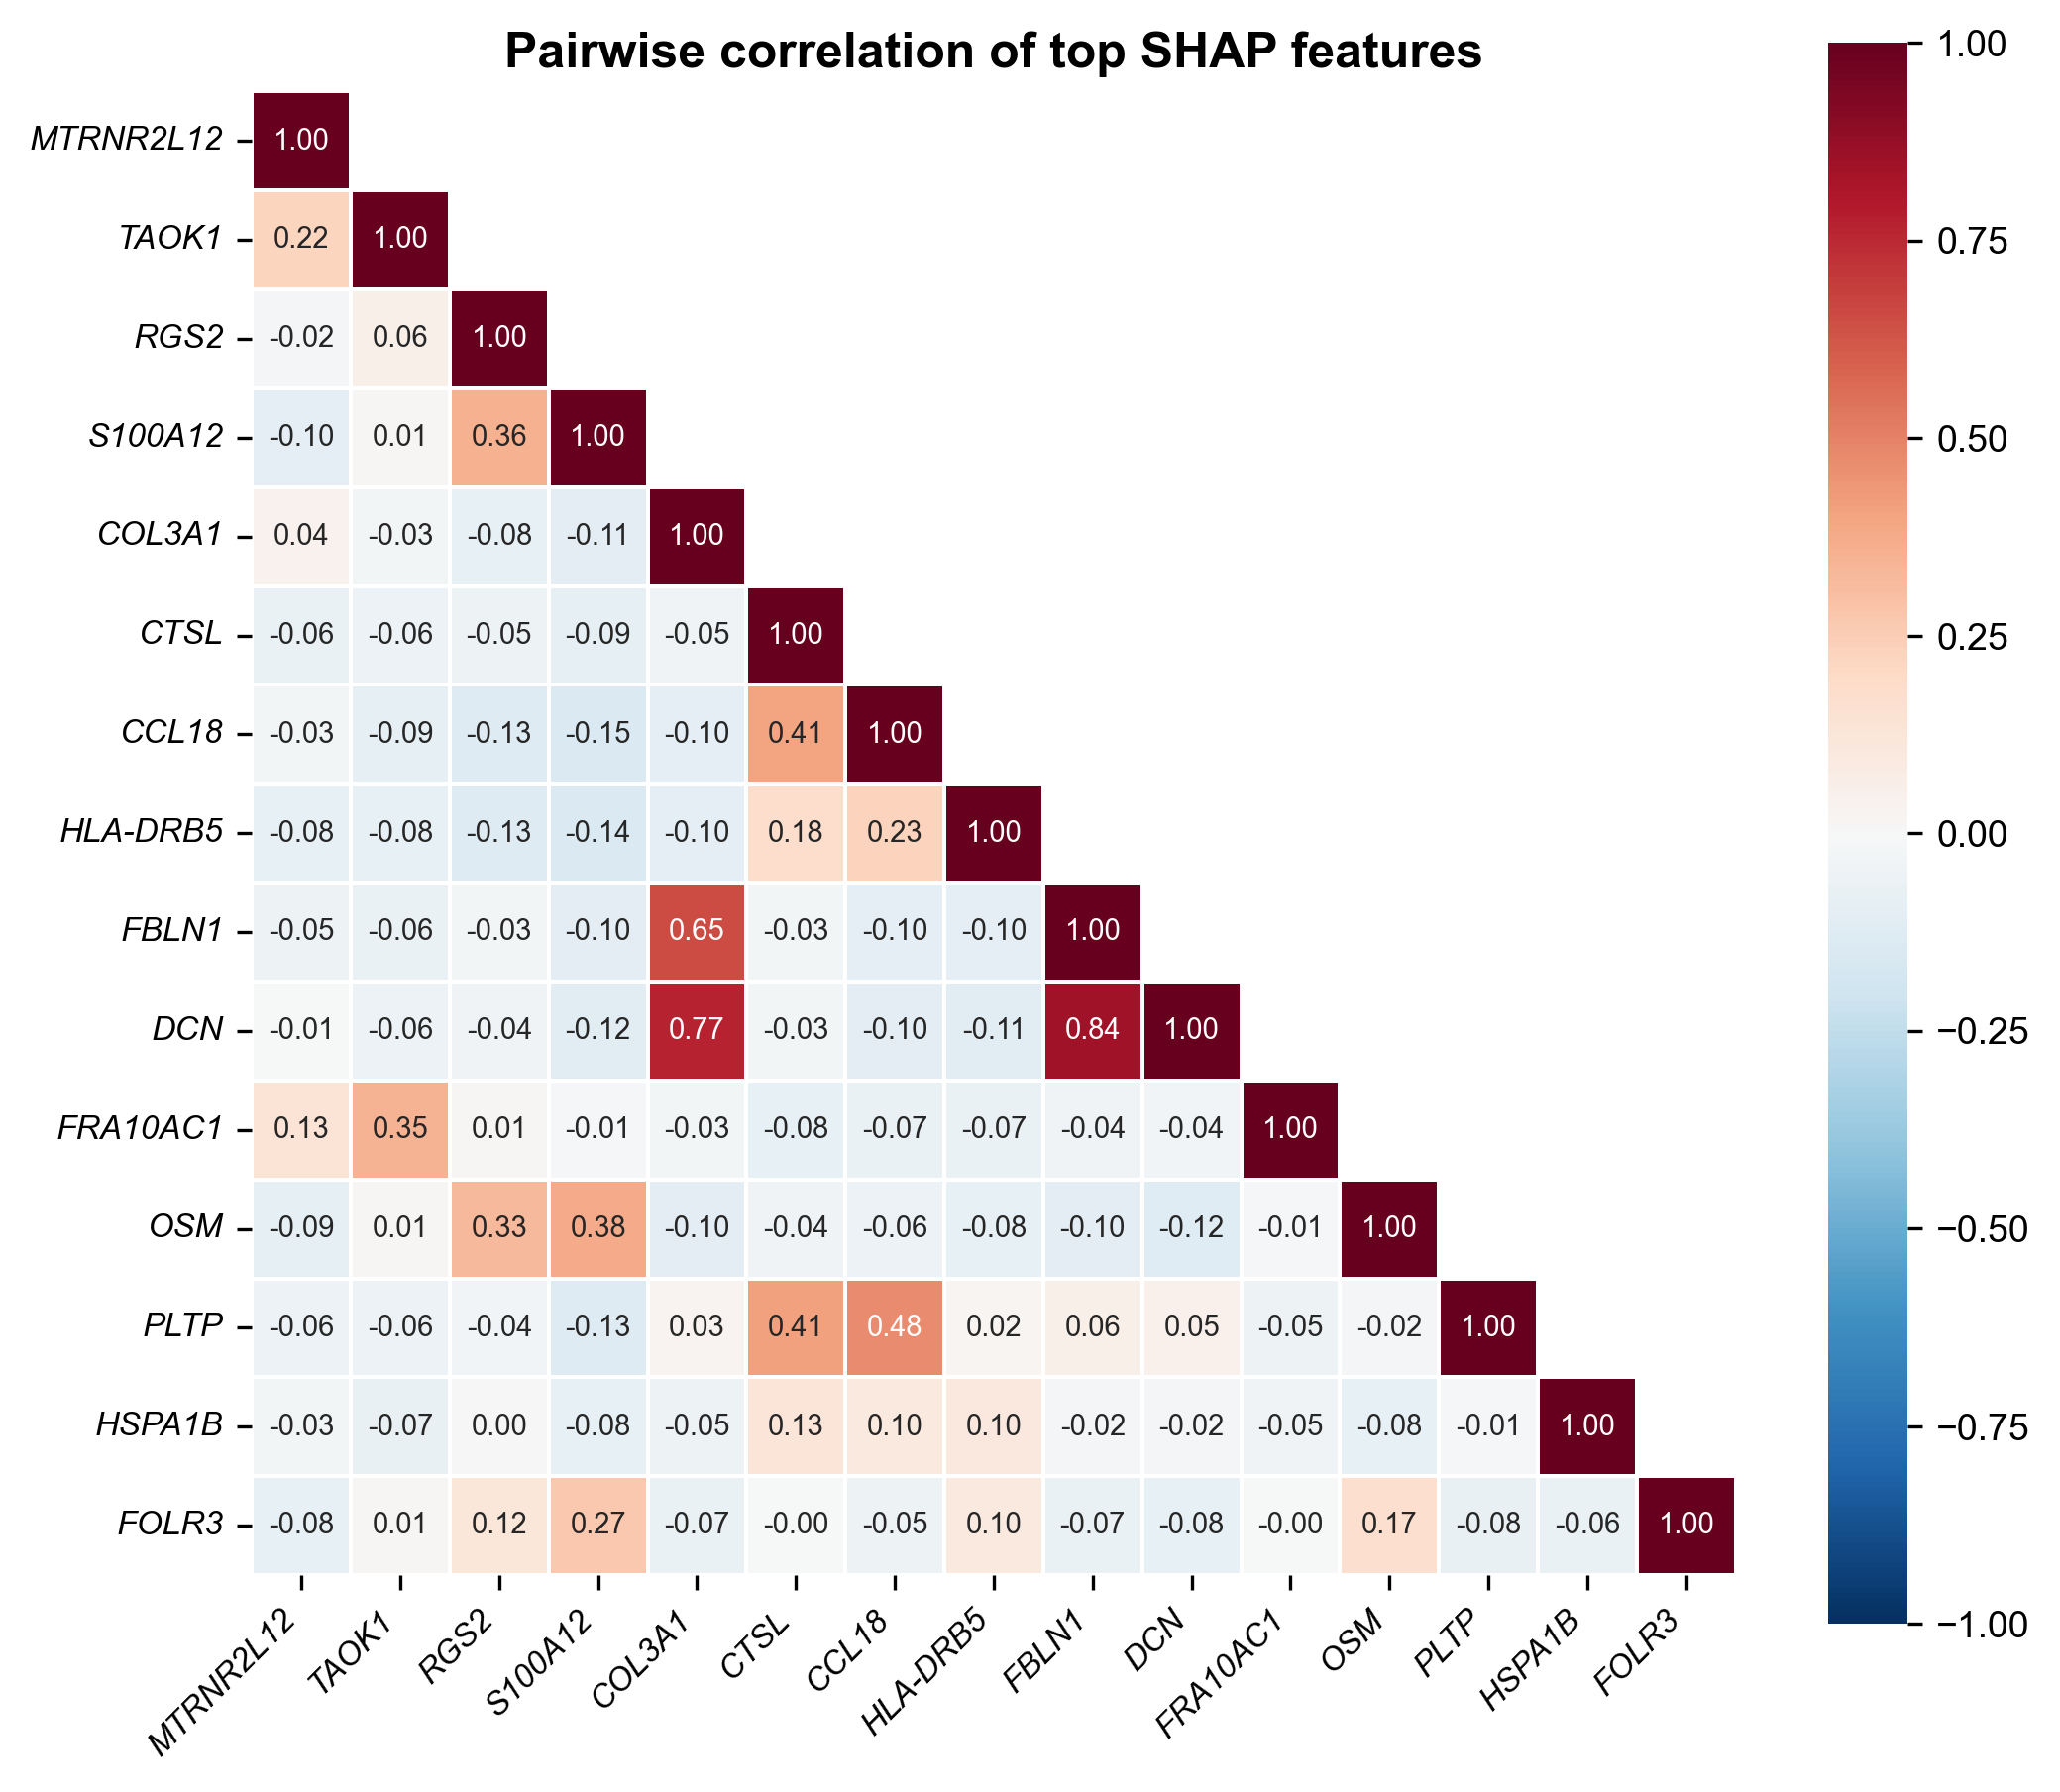
\includegraphics[width=0.85\textwidth]{supp_correlation_matrix.png}
\caption{\textbf{Supplementary Figure S1. Pairwise Pearson correlation matrix of the top 15 SHAP signature genes.} Colour scale ranges from $-$1 (blue, negative correlation) to $+$1 (red, positive correlation). An extracellular matrix module (\textit{COL3A1}, \textit{DCN}, \textit{FBLN1}; pairwise $r \geq 0.65$) and a lipid transport module (\textit{CTSL}, \textit{PLTP}, \textit{CCL18}; pairwise $r = 0.41$--$0.48$) are evident, while most other gene pairs show weak correlations ($|r| < 0.2$), confirming that the disease signature captures largely independent biological programmes.}
\label{fig:suppS1}
\end{figure}

\end{document}
